\documentclass[12pt,a4paper]{article}

\usepackage[german]{babel}
\usepackage[T1]{fontenc}
\usepackage{textcomp}
\usepackage{mathptmx}
\usepackage[utf8]{inputenc}
\setlength{\parindent}{0.0in}
\setlength{\parskip}{0.1in}
\usepackage{amsmath}
\usepackage{amsfonts}
\usepackage{amssymb}
\usepackage{amsthm}
\usepackage{graphicx}
\theoremstyle{definition}
\usepackage{setspace}
\usepackage[left=2.50cm, right=2.50cm, top=2.50cm, bottom=2.50cm]{geometry}
\usepackage{titling}
\newcommand{\subtitle}[1]{%
  \posttitle{%
    \par\end{center}
    \begin{center}\large#1\end{center}
    \vskip0.5em}%
}
\usepackage{hyperref}
\hypersetup{pdfborder=0 0 0}

\usepackage{minted}
\usepackage{enumitem}
\usepackage[nottoc,numbib]{tocbibind}

\title{Verarbeitung Natürlicher Sprache}
\subtitle{Eine Einführung in Theorie und Praxis}
\author{Nikolas C. Göbel}
\date{19. März 2013\\Heinrich-von-Gagern-Gymnasium\\Prüfer: Herr Durdaut}

\begin{document}
\maketitle
\thispagestyle{empty}
\newpage

\tableofcontents
\newpage

\onehalfspacing

\section{Einführung}
	Die Verarbeitung natürlicher Sprache (von nun an: Computerlinguistik oder CL) ist ein Teilgebiet der Informatik, speziell der Künstlichen Intelligenz. Sie verbindet die Informatik mit der Linguistik, zwei Wissenschaften die zunächst vollkommen disjunkt scheinen. Das folgende Kapitel beschäftigt sich damit, welche Probleme die Computerlinguistik zu lösen versucht, sowie mit dem praktischen und gesellschaftlichen Nutzen solcher Technologien.

	\subsection{Problemstellung}
		Maschinen sind exzellente Sortierer, Durchsucher und Berechner. Mit Texten aus dem Alltag, z.B. Zeitungsartikeln oder gesprochenen Befehlen eines menschlichen Nutzers, können sie jedoch erstmal wenig anfangen. Hier kommt die (Angewandte-) Computerlinguistik (englisch: Natural Language Processing, NLP) zum Einsatz. Sie basiert auf linguistischen Formalismen und stochastischen Modellen, mit deren Hilfe die unterschiedlichsten Algorithmen zur Lösung eines Problems erarbeitet werden, welches nun genauer definiert werden soll:

			\newtheorem{nlp}{Definition}[subsection]
			\begin{nlp}
				Die Computerlinguistik beschäftigt sich mit dem Problem, beliebige
				Sätze und Texte in natürlicher Sprache (z.B. Deutsch oder  Englisch) in
				Befehle und Modelle umzuwandeln, die eine Maschine ">verstehen"< und ausführen kann.
			\end{nlp}

		Das Konzept des Verstehens genau zu definieren, ob biologisch oder im maschinellen Kontext, bedarf ausführlicher, auch philosophischer Auseinandersetzungen, welche den Rahmen und den Fokus dieser Arbeit sprengen bzw. verfehlen. Da ein Verstehen im philosophischen Sinne für die praktische Anwendbarkeit der CL (nach aktuellem Stand der Technik) lediglich von begrenztem Nutzen ist, belassen wir es an dieser Stelle bei dem Hinweis. Für obige Definition ">verstehen"< bedeuten, dass die Maschine sinnvoll auf eine Eingabe reagiert, also z.B. eine korrekte Übersetzung liefert, einen Befehl wie verlangt umsetzt oder die richtigen Fakten aus einem Textkörper extrahiert.

	\subsection{Motivation}
		Für einen kurzen Augenblick wollen wir die Lösung des Problems aus 1.1.1 zurückstellen und stattdessen eine Antwort auf die Frage suchen, warum Maschinen menschliche Sprache verstehen lernen sollten. Was für Auswirkungen dieses Verständnis schon heute auf unseren Alltag hat, ist Inhalt des fünften Kapitels.

		Die Computerlinguistik erhält ihre Daseinsberechtigung zunächst aus wissenschaftlicher Sicht: Um einer Maschine beizubringen, natürliche Sprache wie ein Mensch zu verstehen, muss man sich unweigerlich mit der Funktionsweise des menschlichen Sprachverstehens auseinandersetzen. Dessen Entschlüsselung hätte nicht nur Auswirkungen auf die Linguistik, sondern auch auf Biologie, Psychologie und vielleicht sogar Medizin. Auch das Erlernen von Fremdsprachen kann potentiell von Erkenntnissen in diesem Bereich profitieren.

		Für mich persönlich jedoch, wie auch für viele Forscher auf dem Gebiet, gibt es noch einen ganz anderen Grund, maschinelles Sprachverständnis zu verbessern und zu verbreiten. In einer Zeit in der schon Kleinkinder vermehrt das Tablet dem Bilderbuch vorziehen, sind immer noch diejenigen Menschen in der Mehrheit, die zwar Zugang zu Computern besitzen, aber diese nur in sehr begrenztem Maße bedienen können. Viele Benutzer sind spätestens dann der Verzweiflung nahe, wenn das komplizierte Innenleben des Rechners mal einen Aussetzer hat und ein Befehl nicht das gewünschte Resultat liefert. Doch die Schuld an diesem Missstand trägt meistens ein inhärentes Problem von Benutzerschnittstellen.

		Computerprogramme bieten ihren Nutzern eine bestimmte Menge an Befehlen. Diese lassen sich bei einem Getränkeautomaten noch an einer Hand abzählen, doch schon bei einem komplexeren Programm wie Microsoft Word reichen vermutlich alle Finger einer kleinen Stadt nicht mehr aus. Alle möglichen Befehle können also im Allgemeinen nicht auf einmal dem Nutzer präsentiert werden. Die Entwickler einer Software müssen daher zusammenhängende Befehle gruppieren und in irgendeiner Art von Menü anordnen. Es ergeben sich Menü-Hierarchien, die, je nach Komplexität der Anwendung, unhandhabbare Ausmaße annehmen können. Effizientes Arbeiten auf professionellem Niveau, z.B. mit Adobe Photoshop, erfordert oft jahrelanges Training. Einen großen Teil dieser Zeit verbringt der Nutzer mit dem Auswendiglernen der jeweiligen Menü-Hierarchie, um benötigte Befehle schnell erreichen zu können. Die Designer der Software dagegen, müssen einen ständigen Kompromiss zwischen Bedienbarkeit und Funktionalität eingehen. Die Aufteilung, die sie schlussendlich wählen, muss auch vom Benutzer angenommen werden, was unweigerlich zu unkomfortabler Bedienung führt, nämlich genau dann, wenn sich die Vorstellungen des Nutzers, wo ein bestimmter Befehl aufzufinden sei, von der des Designers abweicht, wo besagter Befehl am leichtesten vom Nutzer gefunden werden kann. (Grob) Verallgemeinernd könnte man sagen: Je tiefer die Menü-Hierarchie, desto umständlicher die Benutzung, je flacher die Menü-Hierarchie, desto weniger Funktionalität ist verfügbar. Es besteht ein Kommunikations-Problem zwischen Mensch und Maschine, welches bis vor kurzem nur dadurch gelöst werden konnte, dass der Mensch die Struktur der Benutzerschnittstelle verinnerlicht.

		Dieser kognitive Overhead hat zur Folge, dass Menschen, die sich weniger mit Technik beschäftigen, Computer immer noch nicht als natürliches Werkzeug zum produktiveren Arbeiten ansehen (können). Der Siegeszug der ">Apps"<, Anwendungen für mobile Rechner wie Smartphones und Tablets, hat diesen Benutzbarkeitskonflikt nur noch verschärft. Sie haben aufgrund der kleineren Bildschirme viel weniger Platz für Bedienelemente, müssen aber dennoch gute Funktionalität bieten.

		Die Software-Branche ist traditionell ständig auf der Suche nach Möglichkeiten, ihre Programme leichter und intuitiver bedienbar zu gestalten. In den letzten Jahren hat sich eine dieser Möglichkeiten besonders hervorgetan: Natürliche Sprache. Eine auf natürlicher Sprache basierende Benutzerschnittstelle wäre um ein Vielfaches intuitiver und effizienter. Anstatt die Position und Bedeutung von Befehlen lernen zu müssen, spricht der Benutzer einfach in seiner Muttersprache, um mit einem Programm kommunizieren zu können. So entwickelt z.B. die oben erwähnte Firma Adobe in Kooperation mit der Universität Michigan zurzeit eine neue Version der ">Photoshop"<-Software, die mittels Sprachverarbeitung auch Laien die professionelle Bildbearbeitung ermöglichen soll.\footnote{Siehe dazu [Laput et al. 2013]}

		Ausgewählte praktische Anwendungen werden wir in Kapitel 5 näher betrachten.

\pagebreak
\section{Architektur eines Systems zur Sprachverarbeitung}
	Ein flüssiger Dialog zwischen Mensch und Maschine erfordert neben dem eigentlichen Verständnis des Gesprochenen sowohl einen hochentwickelten Spracherkennungs-Algorithmus, als auch eine Möglichkeit, Text in menschlicher Stimme auszugeben (Sprachsynthese). Beides überschreitet die (alleinige) Zuständigkeit der Computerlinguistik und wird nicht Teil dieser Arbeit sein.
	
	\begin{figure}[hbtp]
	\centering
	\label{Architektur eines natürlichsprachigen Systems}
	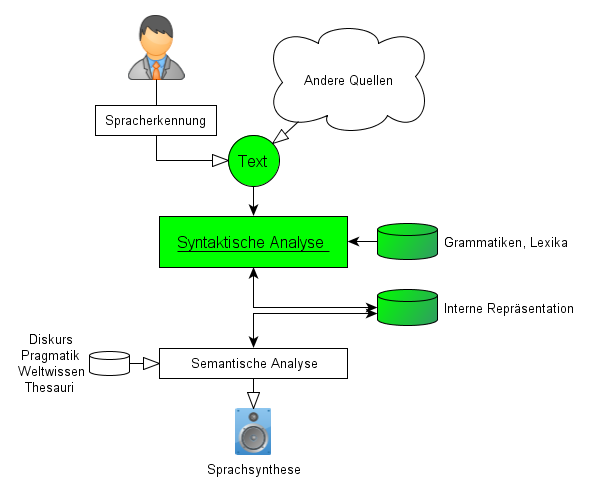
\includegraphics[width=\linewidth]{Grafiken/Architektur}
	\end{figure}
	
	Wir wollen uns auf den nächsten Seiten ausschließlich mit dem grün hervorgehobenen Bereich beschäftigen, einem System, das natürlichsprachigen Text als Eingabe annimmt und mittels Methoden der syntaktischen Analyse in eine interne Repräsentationsstruktur überführt.  Dabei verwendet es Hilfsmittel wie Grammatiken und Lexika, sowie Erkenntnisse aus den bisher analysierten Teilen der Eingabe (daher die rückführenden Pfeile).
	Die syntaktische Analyse behandelt die Morphologie (Wortformen) und die Syntax (Satzstruktur) natürlichsprachiger Eingaben, während die Semantik die Bedeutung einzelner Wörter und deren Einfluss auf die Bedeutung der Eingabe untersucht.

\section{Theoretische Grundlagen}
	Nachdem wir nun geklärt haben, warum sich die Beschäftigung mit maschinellem Sprachverständnis lohnt, wie ein vollständiges natürlichsprachiges System aufgebaut ist und welche Teile wir davon behandeln werden, wenden wir uns in diesem Kapitel den theoretischen Grundlagen der syntaktischen Analyse zu.

	\subsection{Der Parser}
		Die syntaktische Analyse (auch: Parsing) bezeichnet einen Prozess, bei dem eine Zeichenkette (Texte, Symbolketten, Sourcecode,...) nach den Regeln einer formalen Grammatik untersucht wird. Diese Aufgabe übernimmt ein sogenannter Parser. Ein solches Programm transformiert im Allgemeinen eine beliebige Eingabe in ein Format, das besser zur maschinellen Weiterverarbeitung geeignet ist. Für uns ist folgende Definition interessanter:
	
			\newtheorem{Parser}{Definition}[subsection]
			\begin{Parser}
				">Ein Parser in der Computerlinguistik ist ein Automat, der auf Basis einer Grammatik für eine (Zeichen-)Kette einen Ableitungsbaum erzeugt."<
				\footnote{Aus: [Petersen 2010]}
			\end{Parser}

	
		Der Ableitungsbaum (auch Syntaxbaum, engl.: Parse-Tree) zeigt an, welche Ersetzungsregeln der Grammatik zur Erzeugung der Eingabe geführt haben. Er  setzt die Konstituenten eines Satzes in Beziehung. Ein Syntaxbaum ist nützlich um aus einem Satz neue Sätze zu bilden, z.B. einen Aussagesatz in eine Frage umzuwandeln. Allgemein liefert er wertvolle Informationen über die Struktur der Eingabe und ermöglicht z.B. die Identifizierung von Handelnden oder Handlungen im Text. Quasi nebenbei entscheiden Parser das Wortproblem für Sprachen der ihnen zugrunde liegenden Grammatik. Ein valider Ableitungsbaum kann nur dann erstellt werden, wenn die Eingabe von der Grammatik erzeugt wird, also Teil der Sprache ist. Wir werden später jedoch sehen, dass dies nicht die einzige Möglichkeit der syntaktischen Analyse ist. Ein Ableitungsbaum findet sich in Anhang B.1.
	
		\noindent
		Die Funktionsweise eines Parsers lässt sich nach drei Aspekten beurteilen:
			\begin{itemize}
			\item{
				\textbf{Verarbeitungsrichtung:} Die Eingabe kann grundsätzlich von links nach rechts (left-to-right) oder umgekehrt (right-to-left) verarbeitet werden.
			}
			\item{
				\textbf{Analyserichtung:} Der Syntaxbaum kann von der Wurzel ausgehend, in Richtung der Terminale (top-down) oder umgekehrt (bottom-up) erstellt werden. Beim top-down Parsing werden ausgehend von der Wurzel des Baumes (üblicherweise mit S bezeichnet) solange Produktionsregeln angewendet, bis die Eingabe erzeugt wird. Im Gegensatz dazu geht das bottom-up Parsing von den Terminalen (also der Eingabe) aus und ersetzt diese durch umgekehrte Anwendung der Produktionsregeln solange, bis nur noch die Wurzel S übrig bleibt.
			}
			\item{
				\textbf{Suchstrategie:} Wie wir später noch sehen werden, haben Parser (für natürliche Sprachen) es selten mit eindeutigen Grammatiken zu tun. Können an einer Stelle des Baums mehrere Regeln angewendet werden, so bedarf es einer geeigneten Suchstrategie (Heuristik), um aus allen möglichen Pfaden den richtigen zu wählen.	
			}
			\end{itemize}

		\noindent
		Die Komplexität des Parsers hängt sowohl von der letztendlich gewählten Funktionsweise, als auch von der Erzeugungsmächtigkeit der verwendeten Grammatik ab. Ich möchte in dieser Arbeit jedoch von einer anderen Ebene ausgehen, und die  Parser in drei Klassen einteilen: Nichtdeterministisch, Deterministisch und Probabilistisch. Innerhalb dieser Klassen spielen die oben genannten Aspekte natürlich wieder eine Rolle. Ich erhoffe mir von dieser Art der Strukturierung jedoch mehrere Vorteile: Einerseits entspricht sie der geschichtlichen Entwicklung des Feldes, andererseits lassen sich die drei Klassen direkter den unterschiedlichen Theorien der menschlichen Sprachverarbeitung zuordnen. So ermöglicht die gewählte Unterteilung einen einfacheren und intuitiveren Einstieg in das umfangreiche Gebiet der Syntaxanalyse. Zu probabilistischem Parsing muss jedoch ein grober Überblick genügen, da eine detaillierte Einführung den Rahmen dieser Arbeit bei weitem sprengen würde. Doch bevor wir uns den einzelnen Parsing-Methoden zuwenden können, müssen noch einige Grundlagen eingeführt bzw. aufgefrischt werden.

	\subsection{Formale Sprachen und die Chomsky-Hierarchie}
		Um von Maschinen verarbeitet werden zu können, müssen Sprachen und Sprachkonzepte modelliert werden. Mathematik z.B. kann dagegen ">direkt"< von Maschinen benutzt werden, da mathematische Konzepte schon von vornherein formal definiert sind. Ein solches Sprachmodell sind die formalen Sprachen.
	
		Nach der Definition in A.2.3 ist eine formale Sprache also eine Menge aus Wörtern über einem Alphabet. Hier muss zunächst etwas angemerkt werden: Wo natürliche Sprachen sowohl auf Wortebene (Morphologie) als auch auf Satzebene (Syntax) betrachtet werden können, verfügen formale Sprachen nur über eine Ebene, die des Formalen Wortes. Das bedeutet, das bei der Modellierung natürlicher Sprachen durch formale, die Wörter einer formalen Sprache den Sätzen einer Natürlichen entsprechen. ">Peter putzt die Tafel."< wäre also z.B. ein formales Wort der Sprache Deutsch. Alle Wörter einer formalen Sprachen müssen durch ein und dieselbe formale Grammatik erzeugt werden können. Ein Ziel der CL ist es also, natürliche Sprachen möglichst akkurat durch formale Grammatiken zu beschreiben.

		Der US-amerikanische Linguist Avram Noam Chomsky formulierte die nach ihm benannte\footnote{Selten auch \emph{Chomsky-Schützenberger-Hierarchie}, nach M. Schützenberger, französischer Mathematiker mit bedeutenden Beiträgen zur Theorie formaler Sprachen.} Chomsky-Hierarchie zuerst im Jahre 1956\footnote{Siehe [Chomsky 1956]}. Sie teilt die formalen Grammatiken in vier Mächtigkeitsklassen ein (Typ-0 bis Typ-3). Alle Sprachen die von Typ-k Grammatiken erzeugt werden, heißen Sprachen vom Typ-k. Chomsky gilt zurecht als Brückenbauer zwischen Informatik und Linguistik, da seine Hierarchie der formalen Grammatiken einen entscheidenden Beitrag zur Berechenbarkeitstheorie und Komplexitätsanalyse von Automatenmodellen lieferte. Der Zusammenhang zwischen Erzeugungsmächtigkeit eines Grammatikformalismus und der Komplexität des Wortproblems für die erzeugte Sprache, spielt eine wichtige Rolle bei der Suche nach effizienten Algorithmen für die syntaktische Analyse.

		Eine detaillierte Beschreibung der Hierarchie findet sich in [Chomsky 1956] oder [Durdaut 2012]. Hier soll ein grafischer Überblick aus Platzgründen genügen.
		\begin{figure}[hbtp]
		\centering
		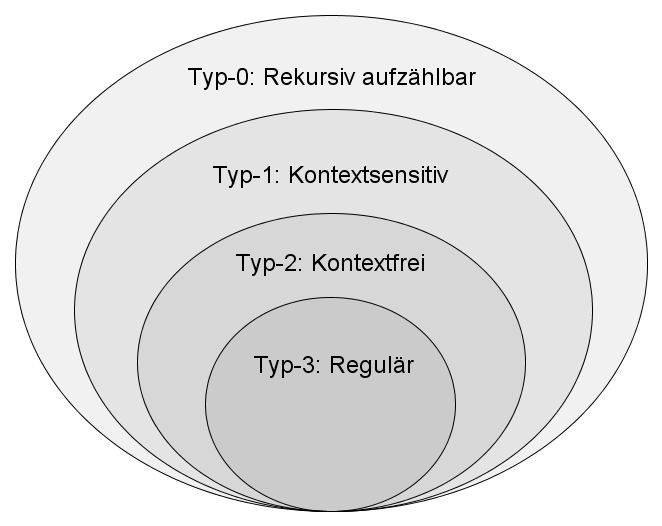
\includegraphics[width=\linewidth]{Grafiken/Chomsky-Hierarchie}
		\end{figure}
	
	\subsection{Die formale Komplexität natürlicher Sprachen}
		Es stellt sich beim Betrachten der Chomsky-Hierarchie die Frage, an welcher Stelle die natürlichen Sprachen eingeordnet werden könnten. Dies ist wichtig, um eine untere Komplexitätsschranke für die syntaktische Analyse bestimmen zu können. So erhält man auch Informationen über die allgemeine Struktur natürlicher Sprachen und kann Rückschlüsse auf menschliche Sprachverarbeitung ziehen. Umgekehrt lässt sich auch feststellen, dass Menschen natürliche Sprache offenbar sehr schnell parsen können, wonach die erzeugenden Grammatikformalismen nicht allzu komplex sein dürften.
	
		\subsubsection{Einordnung natürlicher Sprachen in die Chomsky-Hierarchie}
			Wir wollen aber zuerst einmal klären, ob natürliche Sprachen überhaupt mit formalen Grammatiken beschreibbar sind, also ob wenigstens $\mathit{NL} \subseteq Typ_0$ gilt. Dabei sei $\mathit{NL}$ (Natural Langauges) die Klasse der natürlichen Sprachen. Dies setzt voraus, dass so etwas wie eine Klasse der natürlichen Sprachen überhaupt existiert. Für diese Annahme spricht, dass alle menschlichen Sprachen die gleiche Aufgabe erfüllen und dabei über ähnlich komplexe Ausdrucksmöglichkeiten verfügen, was wiederum auf ähnliche Erzeugungsmächtigkeiten der zugrundeliegenden Grammatiken schließen lässt. Es ist noch anzuführen, dass jeder Mensch eine (Mutter-)Sprache in etwa der gleichen Zeit erlernen kann. Wir können diese Voraussetzung also mit ausreichender Sicherheit als gegeben betrachten.
			
			H. Rogers argumentierte mithilfe der Churchschen These für die formale Beschreibbarkeit der natürlichen Sprachen. Diese besagt, das alles was intuitiv berechenbar ist, auch von Turingmaschinen berechnet werden kann. Da Menschen offensichtlich natürliche Sprache verarbeiten können, müsste dies auch für Turingmaschinen gelten. Da rekursiv aufzählbare Sprachen genau die sind, die von Turingmaschinen akzeptiert werden können, müssten natürliche Sprachen mindestens durch $Typ_0$ Grammatiken formalisiert werden können.
			
			Ich halte einen hybriden Ansatz aus regelbasierten und stochastischen Modellen für am geeignetsten, wie ich im letzten Kapitel dieser Arbeit näher erläutern werde. Diese Vermutung wird laut [Petersen 2006] z.B. durch Theorien R. Matthews gestützt, der sogar gegen die Einschränkung natürlicher Sprachen auf die rekursiv aufzählbaren argumentiert. Nach Matthews basiert menschliches Sprachverständnis ausschließlich auf heuristische Methoden, weswegen wir auch komplexe Sätze effizient parsen, also in Echtzeit verstehen, können. Mit einer solchen Theorie wäre auch die Erlernbarkeit natürlicher Sprachen erklärbar. So kann ein deutscher Muttersprachler durch intensive Lektüre englischsprachiger Texte ein gutes Gefühl für die ">Grammatikalität"< eines englischen Satzes erlangen. Durch das Studium der englischen Grammatik kann er dann für einen Großteil aller englischen Sätze eine eindeutige Antwort bezüglich grammatikalischer Richtigkeit geben. Im Interesse der Allgemeingültigkeit gehen wir zunächst davon aus, dass $\mathit{NL} \subseteq Typ_0$ gilt. Später werden wir uns aber noch mit alternativen Sprachmodellen beschäftigen.
	
			Um eine sinnvolle Einordnung vornehmen zu können, muss an dieser Stelle noch geklärt werden, ob natürliche Sprachen unendliche Mengen sind. Weitere Betrachtungen wären ansonsten nicht nötig, da alle endlichen Sprachen von endlichen Automaten akzeptiert werden können. Doch dies lässt sich schnell zeigen, da durch Konjunktionen oder rekursive Strukturen (wie Nebensatzverschachtelungen) unendlich lange Sätze über einem endlichen Alphabet gebildet werden können. Wir wollen nun also die frisch definierte Klasse NL mit den existierenden Klassen der Chomsky-Hierarchie vergleichen.
			
		\subsubsection{Sind natürliche Sprachen eine Teilmenge der regulären?}
			Diese Vermutung kann mittels des Pumping-Lemmas für endliche Automaten leicht widerlegt werden. Die Durchführung des Beweises findet sich z.B. in [Jäger 2008]. An dieser Stelle wird bereits ein Problem deutlich: Menschen scheinen auch die Sätze in annähernd linearer Zeit verstehen zu können, die beweisen, dass natürliche Sprachen gerade nicht vollständig regulär sind. Ein weiterer Hinweis darauf, dass menschliches Sprachverständnis nicht nur auf formalen Grammatiken basiert?
			
		\subsubsection{Sind natürliche Sprachen eine Teilmenge der kontextfreien?}
			Sei $G$ eine kontextfreie Grammatik $(N, \Sigma, P, S)$, dann ist die von $G$ erzeugte kontextfreie Sprache $L(G) = \{w \in \Sigma^* | S \xrightarrow{*} w\}$.
			
			Kontextfreie Sprachen werden also durch $Typ_2$ Grammatiken erzeugt. Deren Produktionsregeln haben die Form $A \rightarrow \alpha$. Ein Nichtterminal $A$ wird durch eine beliebige Folge an Terminal- und Nichtterminalsymbolen ersetzt. Damit sind KFGs schon erheblich weniger eingeschränkt als reguläre Grammatiken. Mit einer Teilmenge der kontextfreien Sprachen, den deterministisch kontextfreien Sprachen, lassen sich z.B. die meisten Programmiersprachen beschreiben.
			
				\newtheorem{det-cfg}{Definition}[subsubsection]
				\begin{det-cfg}
					Eine Sprache ist deterministisch kontextfrei, wenn es einen  deterministischen
					Kellerautomaten gibt, der sie akzeptiert.
				\end{det-cfg}
			
			Diese sogenannten LR(k)-Grammatiken sind leider im Allgemeinen für das Parsen natürlicher Sprachen nicht ausreichend. Denn natürliche Sprachen unterscheiden sich in einem wichtigen Punkt von den Formalen: Inhärente Mehrdeutigkeiten auf allen Ebenen.
			
				\begin{itemize}
				\item{Phonologisch: ">Adrian hat in Havanna liebe Genossen."<}
				\item{Grammatisch: ">Die Gans schiebt die Mutter in den Ofen."<}
				\item{Semantisch: ">Er liess seinen Freund hängen."<}
				\item{Pragmatisch: ">Es zieht."<}
				\end{itemize}
			
			Mehrdeutige Grammatiken enthalten also für ein oder mehrere Wörter zwei oder mehr unterschiedliche Produktionsregeln. Eine solche Grammatik für ein Fragment des Deutschen findet sich im Anhang B.2.
			
			Intuitiv erfordern allgemein kontextfreie Sprachen also ein (pseudo-)nichtdeterministisches\footnote{Näheres zum nichtdeterministischen Parsen in Kapitel 3.5} Analyseverfahren, dass alle möglichen Regeln ausprobiert und anschließend den richtigen Pfad ermittelt. Durch effiziente Verfahren wie Dynamische Programmierung\footnote{Dieses Verfahren wird in Kapitel 4 kurz erläutert} können kontextfreie Sprachen praxistauglich geparst werden, jedoch sind strikt-deterministische Ansätze immer noch erstrebenswert\footnote{Warum klären wir in Kapitel 3.6}. Einen solchen verfolgt z.B. das PARSIFAL-System von M. Marcus, auf das wir später noch einmal zurückkommen werden. Weiteres zum deterministischen Parsen doppeldeutiger Sprachen findet sich in [Aho et al. 1975].
			
			Natürliche Sprachen galten lange als vollständig kontextfrei. [Bresnan et al. 1982] und [Shieber 1985] konnten jedoch in Form von sogenannten cross-serial dependencies für das Niederländische bzw. Schweizerdeutsche zeigen, dass man nicht alle Aspekte natürlicher Sprache vollständig durch eine kontextfreie Grammatik beschreiben kann. Dennoch werden in der Computerlinguistik häufig KFGs zur Beschreibung natürlicher Sprachen genutzt.
		
		\subsubsection{Sind natürliche Sprachen eine Teilmenge der kontextsensitiven?}
			$Typ_1$ Grammatiken reichen zwar aus, um diese nicht-kontextfreien Bereiche natürlicher Sprachen abzudecken, jedoch ist die erforderliche Komplexität der für kontextsensitive Sprachen benötigten Parser keineswegs wünschenswert\footnote{Mehr dazu in Kapitel 4.2}. Diese Sprachklasse hat damit in der Praxis keine besondere Bedeutung. Es bedarf also, zusätzlich zur Ur-Hierarchie, eines neuen Grammatikformalismus.
		
	\subsection{Schwach-kontextsensitive Grammatiken}
		Um auch die nicht-kontextfreien Aspekte natürlicher Sprachen beschreiben zu können, ohne dabei auf kontextsensitive Grammatiken zurückgreifen zu müssen, wurde die Chomsky-Hierarchie  um eine neue Klasse erweitert. Diese so genannten schwach-kontextsensitiven Grammatiken bilden eine echte Teilmenge der kontextsensitiven und umfassen die kontextfreien. Im unterschied zu den echt-kontextsensitiven Sprachen kann aber das Wortproblem für schwach-kontextsensitive Sprachen in polynomieller Zeit entschieden werden. Erwähnt wurde dieser Grammatikformalismus zuerst in [Joshi 1991]. Man kann auch innerhalb dieser Klasse noch zwischen sehr schwach kontextsensitiven Formalismen (wie z.B. Baumgrammatiken) und mächtigeren, stärker kontextsensitiven unterscheiden. Zu diesen zählen:
		
			\begin{itemize}
			\item{Linear context-free rewriting systems (">lineare, kontextfreie Ersetzungssysteme"<)}
			\item{Minimalist grammars (basiernd auf [Chomsky 1993])}
			\item{Simple-range-concatenation-grammars / SRCGs (">Einfache Intervall-Verkettungsgrammatiken"<)}
			\end{itemize}
		
		Wir beschäftigen uns hier ausschließlich mit den Letztgenannten, da diese in ihrer Struktur am einfachsten verständlich sind. Zunächst betrachten wir die nicht mehr kontextfreie Sprache $L=\{a^nb^nc^n | n \geq 1\}$. Für $L$ existiert keine KFG mehr. Eine SRCG die $L$ erzeugt, kann jedoch mit minimalem Aufwand formuliert werden:
		
			\begin{enumerate}[label={(\arabic*)}]
				\item{$S(XYZ) \rightarrow A(X, Y, Z)$}
				\item{$A(aX, bY, cZ) \rightarrow A(X, Y, Z)$}
				\item{$A(\epsilon, \epsilon, \epsilon) \rightarrow \epsilon$}
			\end{enumerate}
		
		Im Gegensatz zu herkömmlichen Produktionsregeln stehen nun die aus $S$ bzw. $A$ ableitbaren Wörter jeweils in den Klammern dahinter.  Die rechte Seite der Regeln sind für Bedingungen reserviert. Regel (1) besagt also, dass aus $S$ das Wort $XYZ$ abgeleitet werden kann, wenn $X$, $Y$ und $Z$ aus einem Nichtterminal $A$ abgeleitet werden können. $X$, $Y$ und $Z$ heißen Argumente von $A$. Analog formuliert Regel (2), dass aus $A$ drei Teilstrings $aX$, $bY$ und $cZ$ abgeleitet werden können. Diese bestehen jeweils aus einem Terminalsymbol ($a$, $b$ oder $c$) und einem Nichtterminal, welche wiederum aus $A$ ableitbar sein müssen (rechte Seite). Zuletzt besagt Regel (3), dass aus $A$ auch drei leere Teilstrings abgeleitet werden dürfen und zwar bedingungslos (die rechte Seite enthält nur das leere Wort). Im unterschied zu allgemeinen range concatenation grammars gelten für SRCGs folgende Einschränkungen: Während Argumente auf der linken Seite beliebige Folgen aus Terminalen und Nichtterminalen enthalten können, dürfen die auf der Rechten nur aus genau einer Variable bestehen. Zudem müssen die verwendeten Variablen auf beiden Seiten der Regel genau einmal vorkommen.

			\newtheorem{srcg}{Definition}[subsection]
			\begin{srcg}
			Eine SRCG ist ein Tupel $G=(N, \Sigma, V, P, S)$. $N$ ist eine endliche Menge an Nichtterminalen, denen durch die Funktion $dim: N \mapsto \mathbb{N}$ ein Grad zugeordnet wird. $\Sigma$ und $V$ sind disjunkte, endliche Mengen an Terminalsymbolen bzw. Variablen. $P$ ist eine endliche Menge an Produktionsregeln der Form
	
				$$A(\alpha_1, \dots, \alpha_{dim(A)}) \rightarrow A_1(X_1^{(1)}, \dots, X_{dim(A_1)}^{(1)}) \dots A_m(X_1^{(m)}, \dots, X_{dim(A_m)}^{(m)})$$
	
			$S$ ist das Startsymbol. Es gilt $dim(S) = 1$. $G$ heißt k-SRCG wenn gilt:
				
				$$\forall A \in N: dim(A) \leq k$$
			\end{srcg}
		
		Das obige Beispiel zeigt eine dreistellige SRCG (oder 3-SRCG), da die Nichtterminale maximal drei Argumente haben. Das bedeutet, dass im Unterschied zu KFGs, bis zu drei Teilstrings aus einem Wort abgeleitet werden können. Es ist sofort ersichtlich, dass KFGs eine Teilmenge der SRCGs darstellen, nämlich genau die Menge der einstelligen SRCGs. Näheres zur Komplexität des Parsing-Problems für SRCGs findet sich in Kapitel 4.3.
		
	\subsection{Nichtdeterministisches Parsing}
		Wie in Kapitel 3.3.3 angesprochen enthalten formale Grammatiken für natürliche Sprachen fast unweigerlich Doppeldeutigkeiten\footnote{Ein Beweis für die Existenz inhärent mehrdeutiger Sprachen findet sich in [Wegener 1999].}. Das heißt, dass ein Parser für solche Grammatiken Zustände enthält, in denen mehrere alternative Ableitungsschritte möglich sind. Unweigerlich fühlt man sich an dieser Stelle an nichtdeterministische Turingmaschinen erinnert. Diese wählen in solchen mehrpfadigen Zuständen immer richtig, obwohl sie keinerlei Hinweise darüber bekommen ob ihre Entscheidung auch zielführend ist. Leider existieren solche Orakel-Maschinen nur in der Theorie. Nichtdeterministisches Verhalten kann aber sehr wohl von deterministischen Maschinen simuliert werden, denn egal wie viele verschiedene Möglichkeiten es in jedem Schritt gibt, so kann doch eine deterministische Maschine jede einzelne Alternative nacheinander ausprobieren. Mittels des sogenannten Backtrackings wird eine Zustandsfolge solange ausprobiert, bis sie entweder in einem akzeptierenden Zustand endet oder nicht. In letzterem Fall wird die Folge verworfen und die nächste ausprobiert. Ein solches Vorgehen würde intuitiv zu den mehrdeutigen Grammatiken natürlicher Sprachen passen. Doch ist ebenfalls ersichtlich, dass schon bei wenigen Doppeldeutigkeiten die benötigte Rechenzeit stark anwächst. Es gilt:
	
			\newtheorem{simulated-nt}{Satz}[subsection]
			\begin{simulated-nt}
				Eine deterministische Turingmaschine kann eine Nichtdeterministische mit maximal exponentiellem Aufwand simulieren\footnote{Beweis: Siehe [Durdaut 2012] S. 47}.
			\end{simulated-nt}
	
		In der Praxis existieren jedoch dank dynamischer Programmiertechniken auch effiziente, nichtdeterministische\footnote{Nichtdeterministisch steht hierbei natürlich für simulierten Nichtdeterminismus.} Parser, die wir in Kapitel 4 kennenlernen werden.
	
	\subsection{Deterministisches Parsing}
		Nichtdeterministische Parser stellen zwar eine intuitiv ersichtliche Lösung für den Umgang mit Doppeldeutigkeiten dar. Dennoch wäre ein strikt deterministisches Parsen von natürlichen Sprachen, falls möglich, eine erhebliche Erleichterung bezüglich Komplexität und Implementierungsaufwand. Überdies würde ein deterministischer Parser eine inkrementelle Verarbeitung  der Eingabe ermöglichen. Dies wäre besonders interessant für Echtzeit-Analysen (z.B. in der Spracherkennung), bei denen mit jedem neuen Token die gesamte bisherige Analyse aktualisiert werden muss. Auch gibt es psycholinguistische Hinweise darauf, dass das menschliche Gehirn Sprache inkrementell verarbeitet, siehe dazu [Nivre 2004].
	
		Ein deterministischer Algorithmus liefert zu gleichen Eingaben immer die gleiche Ausgabe und durchläuft dabei auch immer die gleiche Folge an Zuständen. Wie bei einem Rezept oder einer Bedienungsanleitung, ist zu jedem Zeitpunkt der Berechnung klar, was der nächste Schritt sein muss. Daraus folgt:
	
			\newtheorem{det-parser}{Satz}[subsection]
			\begin{det-parser}
				Ein Parser operiert deterministisch, wenn in jedem Zustand nur ein Ableitungsschritt möglich ist\footnote{Beweis: Trivial.}.
			\end{det-parser}
	
		Um dennoch mit Doppeldeutigkeiten umgehen zu können, schieben deterministische Parser die Entscheidung für einen Pfad auf, anstatt einfach alle auszuprobieren. Diese Technik nennt sich lookahead oder umgekehrt auch wait \& see. Das Streben nach deterministischen Parsern hat seinen Ursprung größtenteils in der Arbeit von M. Marcus, dessen Algorithmus wir ebenfalls in Kapitel 4 behandeln werden.
	
	\subsection{Probabilistisches Parsing}
		Formale Grammatiken sind nicht die einzige Möglichkeit, Sprachen für Maschinen verständlich zu modellieren. Während formale Sprachen, wie in Kapitel 3.2 besprochen, als eine Wortmenge definiert sind\footnote{Erinnerung: Formale Worte entsprechen den Sätzen einer natürlichen Sprache.}, nämlich genau diejenigen die von der zugrundeliegenden Grammatik erzeugt werden können, verfolgen die sogenannten stochastischen Sprachmodelle einen ganz anderen Ansatz: Sie versuche anhand von Wahrscheinlichkeiten Rechenschritte einzusparen. Eine Möglichkeit ist die Verwendung probabilistisch-kontextfreier Grammatiken\footnote{Ein Beispiel findet sich in Anhang B.3}, bei denen jeder Ableitungsregel eine Wahrscheinlichkeit zugeordnet ist. Anhand dieser können bestehende Algorithmen effizienter implementiert werden. Es ist ohne weiteres Möglich einen strikt-deterministisch operierenden, probabilistischen Parser zu konstruieren, wobei dieser im Allgemeinen nicht den global wahrscheinlichsten Ableitungsbaum liefern wird.
	
		Auch probabilistische Ansätze entsprechen einigen Theorien über die menschliche Sprachverarbeitung, siehe dazu [Chater und Manning 2006] sowie [Hale 2001]. Um den Umgang mit unsicheren Eingaben (z.B. das nicht immer korrekte Ergebnis einer Spracherkennung), muss man sich nun nicht mehr kümmern, ein probabilistischer Parser kann hier sogar Fehler in der Eingabe ausgleichen.

\section{Die Komplexität des Parsing-Problems}
	Nachdem wir nun die verschiedenen Parse-Theorien kennengelernt haben, wollen wir in diesem Kapitel einige Implementationen genauer untersuchen, die das in 3.1 aufgestellte Parsing-Problem lösen.
	
	\subsection{Für kontextfreie Sprachen}
		Für kontextfreie Sprachen kann das Wortproblem in polynomieller Zeit entschieden werden. Das bedeutet wiederum, dass alle Programmiersprachen sowie ein großer Teil der natürlichen Sprachen effizient geparst werden können. Wir betrachten nun zunächst zwei weit verbreitete Varianten des Chart-Parsing, einer geläufigen Methode zur Implementierung nichtdeterministischen Parser. Chart-Parsing bezeichnet eine Methode, bei der bereits berechnete Substrukturen des Ableitungsbaums in einer Datenstruktur, der sogenannten Chart gespeichert werden. Anschließend wenden wir uns noch einem strikt-deterministischen Parser zu, dem Marcus-Parser.
		
		\subsubsection{Der Earley-Parser}
			Der Earley-Parser ist ein top-down operierender, vorausschauender Chart-Parser, der sich dynamische Programmierung zunutze macht. Sein Erfinder, Jay Earley, stellte ihn zuerst in seiner Dissertation [Earley 1968] vor. Der Algorithmus ist in der Praxis sehr beliebt, da er das effiziente Parsen allgemeiner kontextfreier Sprachen ermöglicht. Mit dynamischer Programmierung ist gemeint, dass mehrfach auftretende Teilprobleme nur einmal berechnet werden müssen.
		
			Der Algorithmus speichert Erkenntnisse zur Laufzeit in sogenannten State-Sets (Zustandsmengen). Ein Zustand wird dabei durch ein 4-Tupel $Z=(P, i, l, s)$ beschrieben. $P$ ist dabei eine Produktionsregel aus $G$, deren rechte Seite eine mögliche Ableitung im derzeitigen Zustand darstellt. Der Parser befindet sich am $i$-ten Symbol dieser Regel. Die nächsten k-Symbole sind im Wort $l$ gespeichert. Zuletzt gibt der Set-Index $s \in \mathbb{N}$ an, aus welcher Menge dieser Zustand hervorging (der sogenannte \textit{origin}). Drei Subroutinen laufen nun über alle Zustände in der aktuellen Menge: 
			
			\begin{enumerate}
			\item{
				Der \textit{predictor} (Vorhersager) ist auf alle Zustände anwendbar, für die die rechte Seite von $P$ an der Position $i$ ein Nichtterminal $N$ enthält. Er fügt nun für alle auf $N$ anwendbaren Regeln aus $G$ einen neuen Zustand in das aktuelle Set.
			}
			\item{
				Der \textit{scanner} ist auf alle Zustände anwendbar, bei denen an der Position $i$ in $P$ ein Terminal $T$ steht. Wenn $T$ mit dem nächsten Symbol der Eingabe übereinstimmt, wird der Zustand in die nächste Zustandsmenge $S'$ eingefügt.
			}
			\item{
				Für alle Zustände die am Ende ihrer Produktionsregel $P$ angelangt sind und deren $k$-lookahead mit den nächsten $k$ Symbolen der Eingabe übereinstimmt, fügt der \textit{completer} (Vervollständiger) nun alle Zustände aus dem origin in die neue Menge $S'$ ein. Ist nach dem Durchlauf des completers $S'$ leer, so gehört das Eingabewort nicht zu $L(G)$.
			}
			\end{enumerate}
			
			Bildlich betrachtet konstruiert der Algorithmus also alle Möglichen Ableitungen (predictor), testet welche von den resultierenden Wörtern auf die Eingabe passen (scanner) und reduziert die zu untersuchenden Pfade auf diejenigen, die zu den passenden Wörtern geführt haben (completer). Befindet sich nun in der letzten Zustandsmenge ein einziger Zustand (nämlich der Ausgangszustand), so würde das bedeuten, dass das Startsymbol von $G$ zu der Eingabe geführt hat. Ergo ist die Eingabe in $L(G)$\footnote{Ein Schritt-für-Schritt Beispiel findet sich hier: http://en.wikipedia.org/wiki/Earley\_parser\#Example}. Meine Implementation eines Earley-Akzeptors liegt im Anhang C.2 bei.

			Allgemeine kontextfreie Sprachen können in $O(n^3)$ erkannt werden. $n$ sei hierbei die Länge der Eingabe. Für eindeutige und beschränkt mehrdeutige Grammatiken reduziert sich die Laufzeitskomplexität auf $O(n^2)$, für viele LR(k)-Grammatiken sogar auf $O(n)$. Diese Komplexitäten ergeben sich wie folgt:
			
			Der Algorithmus benötigt ein State-Set für jede Position der Eingabe $w$. Es gilt $|w|=n$, damit ist die Anzahl State-Sets gegeben durch $n+1$, bzw. $O(n)$. Für uneingeschränkt mehrdeutige Grammatiken kann der predictor höchstens $O(n*|G|)$ Zustände erzeugen. Der aufwendigste Schritt, der completer, muss für die $O(n*|G|)$ Zustände im aktuellen Set alle Zustände eines vorherigen überprüfen, also höchstens $O((n*|G|)^2)$. Daraus folgt:
				
				$$O(n)*(O(n*|G|)+O(n^2*|G|^2)) = O(n^3*|G|^2)$$
			
			Die Platzkomplexität wird allgemein durch $O(n^2*|G|)$ beschränkt, $O(n*|G|)$ Zustände in $O(n)$ State-Sets. Alle Angaben entsprechen der Original-Analyse Earleys in [Earley 1968]. Zur Platzkomplexität findet sich in [Li und Alagappan 2009] eine widersprüchliche Angabe von $O(n)$. Diese gilt meinem Verständnis nach aber nur für beschränkt mehrdeutige Grammatiken und lässt mit der Vereinfachung von $O(n*|G|)$ zu $O(|G|)$ außer Acht, dass durchaus dieselbe Regel in mehreren Zuständen vorkommen kann.
		
		\subsubsection{Der Coke-Younger-Kasami-Parser}
			Im Unterschied zum Earley-Parser setzt der CYK-Algorithmus eine Grammatik in CNF (Chomsky-Normalform) voraus. Dies ist bei Betrachtung der Beschreibungskomplexität ein Nachteil. Allgemeine Kontextfreie Grammatiken G können in  $O(n^3)$ analysiert werden. Für einen Großteil der Anwendungen ist der Earley-Parser jedoch effizienter. Strukturell arbeitet der CYK-Parser bottom-up, daher müssen keine Vorhersagen getroffen werden und die predictor-Komponente entfällt.
		
			Der Platzbedarf des CYK-Algorithmus wird, wie der Earley-Parser, durch $O(n^2)$ beschränkt. Zeit- und Platzkomplexität sind in [Li und Alagappan 2009] festgehalten und experimentell überprüft worden.
		
		\subsubsection{Der Marcus-Parser}
			Der Marcus-Parser (ursprünglich: PARSIFAL-System) ist ein deterministischer, vorausschauender Parser. Vorausschauend bedeutet hierbei, dass der Parser zur Verarbeitung des aktuellen Tokens die folgenden $n$ Token miteinbeziehen darf. In der ursprünglichen Implementierung aus [Marcus 1980], wird $n=3$ gesetzt. Marcus Arbeit basiert auf seiner Determinismus-Hypothese:
		
				\newtheorem{det-hypothesis}{Satz}[subsubsection]
				\begin{det-hypothesis}
					">The syntax of any natural language can be parsed by a mechanism which operates ">strictly deterministically"< in that it does not simualte a nondeterministic machine."<\footnote{Entnommen aus: [Marcus 1980] Kapitel 1.1}
				\end{det-hypothesis}
				
		
			Nach Marcus ist es also möglich, einen Parser zu konstruieren, der ohne simulierten Nichtdeterminismus mit mehrdeutigen Grammatiken umgehen kann. Er wollte genau diesen ">Halbdeterminismus"< vermeiden, um von den Effizienzvorteilen einer strikt-deterministischen Lösung profitieren zu können. Dazu postulierte er drei Regeln, die solch ein Parser einhalten müsse:
		
				\begin{enumerate}
				\item{\textbf{Kein Backtracking.} Alle Teile des Syntaxbaums, die der Parser schon generiert hat, dürfen nichtmehr verändert werden.}
				\item{
					\textbf{Keine parallelen Strukturen.} Alle syntaktischen Substrukturen, die der Parser generiert, müssen Teil der Ausgabe sein. Somit wird verhindert, dass der Parser Nichtdeterminismus durch parallele Verarbeitung mehrerer möglicher Strukturen simuliert.
				}
				\item{\textbf{Keine versteckten Zustände.} Das bedeutet, dass der Parser keine temporär erzeugten Strukturen in seinem Zustand kodieren darf.}
				\end{enumerate}
		
			Marcus' Implementation operiert left-to-right und top-down. Die nächsten möglichen Regeln werden jedoch bottom-up, also von der Eingabe ausgehend, gesucht. Der Parser nutzt zwei Datenstrukturen, einen Stack aktiver Teilstrukturen und einen $n$-stelligen Puffer. Letzterer enthält die nächsten $n$ Symbole der Eingabe (lookahead) bzw. vollständig erkannte Teilstrukturen, da alle Strukturen (in einem top-down Parser) nur von einem Terminal abgeschlossen werden können.
		
			Aus der Grammatik wird nun, beginnend mit dem Startsymbol, immer die nächste erwartete Konstituente bestimmt. Ist diese eindeutig, existiert also nur eine anwendbare Regel für das aktuelle Symbol, so wird das nächste Symbol der Regel in den Erwartungsstack eingefügt. Existieren jedoch mehrere Produktionsregeln für das aktuelle Symbol, so wird der Inhalt des Puffers betrachtet, um die richtige Regeln zu identifizieren. Erkennt der Parser bei einer solchen Puffer-Analyse ein Terminal, dass die aktuelle Teilstruktur abschließt, so nimmt er die nun vervollständigte Struktur vom Stack und ersetzt das Terminal im Puffer durch sie. Gehört die Eingabe zur Sprache, so bleibt am Ende des Vorgangs ein leerer Puffer und ein einziges Element auf dem Stack, das den vollständigen Ableitungsbaum enthält. Ein beispielhafter Durchlauf findet sich in Anhang B.4.
		
			Interessant ist auch die Herangehensweise an grammatikalische Sonderfälle. Der Parser unterteilt Grammatikregeln in Pakete, von denen zu jedem Zeitpunkt mehrere aktiv sein können. Aktive Pakete werden dann in jedem Zustand auf anwendbare Regeln durchsucht. Dies spiegelt die grundlegende Idee hinter dem PARSIFAL-System wider: Eine Vielzahl an Möglichkeiten durch intelligentes Einschränken handhabbar machen.
		
			Der ursprüngliche Parser wurde inzwischen mehrfach verbessert oder erweitert, eine  bekannte Implementierung ist Fidditch von [Hindle 1983], mit dessen Hilfe die Penn-Treebank erstellt wurde. Auch existieren Variationen wie [Covington 1990], die besser für die Analyse von Sprachen mit freier Wortstellung (wie z.B. Latein) geeignet sind. Meine Implementation liegt im Anhang C.1 bei.

	\subsection{Für kontextsensitive Sprachen}
		Das Wortproblem für allgemeine kontextsensitive Sprachen ist NP-Vollständig, also nicht effizient entscheidbar ($P \neq NP$ vorausgesetzt). Die in 4.1 vorgestellten Algorithmen für kontextfreie Sprachen, lassen sich zwar auf kontextsensitive Grammatiken ausweiten, dabei verlieren aber die Laufzeitbetrachtungen ihre Gültigkeit. In der Praxis ist die Analyse des Wortproblems für schwach-kontextsensitive Sprachen von größerer Bedeutung.
	
	\subsection{Für schwach-kontextsensitive Sprachen}
		Für schwach-kontextsensitive Sprachen kann keine allgemein gültige Komplexitätsanalyse durchgeführt werden, da (wie in 3.4 besprochen) unterschiedlich mächtige schwach-kontextsensitive Grammatikformalismen existieren. Es ist nicht klar ob über den bekannten SKSGs noch mächtigere PTIME\footnote{PTIME ist hierbei die Klasse aller in maximal polynomieller Zeit analysierbaren Grammatiken} Grammatikklassen liegen, SRCGs sind aber dank ihrer nähe zu den allgemeinen RCGs, welche schon außerhalb von PTIME liegen, ein vielversprechender Kandidat. Das Wortproblem für k-SRCGs kann also in polynomieller Zeit entschieden werden, die Laufzeit steigt jedoch exponentiell mit $k$ an. Eine Version des inkrementellen Earley-Parsers, vorgestellt in [Kallmeyer und Maier 2009],  kann allgemeine SRCGs effizient parsen.
	
		Für einen umfassenden Überblick über das Parsen aller geläufigen SKS-Sprachklassen siehe [Kallmeyer 2010].
	
	\subsection{Für probabilistische Sprachmodelle}
		Probabilistische Parser sind meist verallgemeinerte Algorithmen für KFGs, die mit den Wahrscheinlichkeiten einer PKFG umgehen können. Der Earley-Parser kann z.B. mit geringem Aufwand auch PKFGs verarbeiten, wobei vor allem die predict und complete Schritte profitieren. Dabei bleibt allerdings die generelle Struktur des Parser erhalten, weswegen sich die Komplexitäten nicht verbessern. Lediglich die einzelnen Schritte werden effizienter.\footnote{Eine detailliertere Analyse ist aus Platzgründen leider nicht möglich, bei Interesse liefert [Stolcke 1995] jedoch einen guten Einstieg.}

\section{Gesellschaftliche Relevanz}
	Abgesehen von dem hohen Nutzen den die heutzutage noch relativ begrenzten computerlinguistischen Fähigkeiten vieler Systeme bieten (z.B Spam-Filter oder Suchmaschinen), zeigt die Forschung in diesem Gebiet neue, noch interessantere Perspektiven auf: Um den vollen Nutzen aus Maschinen ziehen zu können, muss der Nutzer immer noch einen großen Lernaufwand vollbringen. Die Programmierung einer Maschine erfordert vielfältige Kenntnisse, nicht nur der eigentlichen Programmiersprache, sondern auch der internen Abläufe auf Hardware-Level. Um die Vorteile von Rechnern möglichst vielen Menschen zu eröffnen, haben fähige Leute in den Letzten Jahrzehnten immer neue, verbesserte Interfaces erdacht, die immer mehr Möglichkeiten auf einfache und schnell erlernbare Weise zugänglich machen.

	Im Grunde ist natürliche Sprache, im Bezug auf Maschinen, nichts als eine weitere Schnittstelle für den Benutzer. Doch hat sie einen entscheidenden Vorteil gegenüber allen anderen Bedienmöglichkeiten: Jeder Nutzer beherrscht sie. Jeder Nutzer kann in seiner Sprache ausdrücken was er erreichen will, aber dies nicht immer einer Maschine verständlich machen. CL erlaubt es uns, diese Lücke zu schließen, und Computer wirklich allen Menschen zugänglich zu machen.
	
	\subsection{Anwendungsbereiche Heute}
		Das in 1.2 angesprochene, ultimative Ziel einer vollständig natürlichen Kommunikation zwischen Mensch und Maschine rückt zwar beständig näher, ist jedoch noch lange nicht erreicht. Doch eine Maschine muss natürliche Sprache nicht immer in allen Aspekten verstehen um nützlich zu sein. Ganz im Gegenteil hat CL heute schon großen Nutzen und ist zudem schon weiter im Alltag verbreitet als viele Menschen vielleicht glauben. Einige der wichtigsten Einsatzbereiche sind:

		\begin{itemize}
		\item{
			\textbf{Spam-Filter:}
			Bestimmte CL-Algorithmen, sogenannte Classifier, können anhand des Inhalts einer Mail bestimmen, wie wahrscheinlich sie Spam enthält. Dazu wird vorher aus Analysen von tausenden, als Spam bekannter Mails, ein statistisches Modell errechnet. Solche Classifier haben aber darüber hinaus unzählige weitere Nutzen. So beschreibt z.B. [Mukherjee et al. 2012] eine Methode um gefälschte Produkt-Rezensionen zu erkennen.
			
		}
		\item{
			\textbf{Suchmaschinen:}
			Traditionell liefern Suchmaschinen nur Ergebnisse, die bezüglich bestimmter Schlüsselwörter mit der Eingabe des Users übereinstimmen. Seit einiger Zeit versuchen aber viele Anbieter Suchanfragen auch inhaltlich zu verstehen, um möglichst direkte Antworten liefern zu können. Sucht man z.B. mit Google nach ">Wie alt ist Noam 	Chomsky?"< oder ">Wie hoch ist der Eiffelturm?"<, so erhält man neben den obligatorischen Links zu Wikipedia und Konsorten auch ein großes Textfeld mit der 	entsprechenden Antwort, ohne weitere Seiten besuchen zu müssen. Ein Beispiel liegt im Anhang B.5 bei.
		}
		\item{
			\textbf{Automatische Übersetzung / Zusammenfassung:}
			Eine der schwersten Disziplinen der CL ist die automatische Übersetzung von Texten, denn sie erfordert nicht nur ein tiefes grammatikalisches Verständnis der Quellsprache, sondern auch die Fähigkeit grammatikalisch richtige Sätze in der Zielsprache zu formulieren, ohne dabei den ursprünglichen Sinn zu verändern. Ähnlich kompliziert ist das automatische Zusammenfassen von Texten.
		}
		\item{
			\textbf{Virtuelle Assistenten:}
			Dank ">Siri"<, der virtuellen Assistentin in Apple's iPhones, sind sie heute populär wie nie zuvor: Virtuelle Assistenten, die Verwirklichung des großen Ziels der Computerlinguistik. Sie versprechen annähernd menschliche Kommunikation mit einer Maschine und viele der Annehmlichkeiten, die ein menschlicher Sekretär bietet: Termine eintragen und rechtzeitig an diese erinnern, die neuesten Bundesliga-Ergebnisse liefern, Reservierungen in Restaurants vornehmen oder Kinokarten kaufen. Doch genauso ist dank ">Siri"< vielen Menschen wieder klar geworden, dass solche Technologien noch sehr unausgereift sind und zudem weit davon entfernt, einen menschlichen Assistenten ersetzen zu können. Dies liegt daran, dass heutige virtuelle Assistenten gesprochene Befehle nicht wirklich verstehen, sondern nur in bestimmte Kategorien, wie Wetter, Sportergebnisse oder Restaurant-Suche einordnen können. Entspricht die Formulierung des Benutzers einmal nicht den Erwartungen, sind solche Systeme schnell überfordert. Dennoch macht auch die Entwicklung in diesem Bereich jedes Jahr große Sprünge nach vorne.
		}
		\end{itemize}
		
		Hinzu kommen hunderte weitere Anwendungen, von der automatischen Essay- oder Arbeiten-Korrektur, bis hin zu Systemen, die selbstständig tausende Bücher schreiben und verkaufen\footnote{http://singularityhub.com/2012/12/13/patented-book-writing-system-lets-one-professor-create-hundreds-of-thousands-of-amazon-books-and-counting/ , [Stand: 04.02.2013]}.

	\subsection{Nutzen in der literarischen Analyse}
		Die Idee, dass natürliche Sprachen durch statistische Modelle beschrieben werden können, brachte frischen Wind in ein Gebiet, das faszinierende Einblicke in unsere Gesellschaft liefern kann: Literarische Analyse. Traditionell war diese immer auf einzelne, als wichtig geltende Werke einer Epoche beschränkt. Heutige Rechner, gepaart mit Erkenntnissen der Computerlinguistik, erlauben weitaus umfassendere Untersuchungen. So stellt z.B. der Suchmaschinen-Anbieter Google, für jedermann frei verfügbar ein Online-Tool\footnote{Google Ngram Viewer - http://books.google.com/ngrams} bereit, mit dem die Verwendungshäufigkeit pro Jahr von beliebigen Phrasen, grafisch dargestellt werden kann. Das Programm greift dabei auf Googles Datenbank aus knapp 5.1 Millionen gescannten Büchern in mehreren Sprachen zu\footnote{http://en.wikipedia.org/wiki/Google\_Ngram\_Viewer [Stand: 2008]}. Die Mächtigkeit solcher Recherchen möchte ich an einigen Beispielen demonstrieren, siehe dazu Anhang B.6.
	
		Andere, höchst-aktuelle Studien untersuchen welche Autoren den größten Einfluss auf die Literatur ihrer und nachfolgender Generationen hatten\footnote{http://www.nytimes.com/2013/01/27/technology/literary-history-seen-through-big-datas-lens.html [Stand: 04.02.2013] - Studie (noch nicht erschienen): M.L. Jockers (2013): \emph{Macroanalysis. Digital Methods and Literary History.}}. [Jockers 2013] entdeckte z.B., dass nicht etwa Charles Dickens oder Mark Twain, sondern Jane Austen und ">Ivanhoe"< Autor, Sir Walter Scott die größten Einflüsse auf englischsprachige Literatur hatten.

\section{Ergebnis}
	Wir haben nun einen Überblick über die theoretische, sowie die Auswirkungen der praktischen Computerlinguistik gewonnen.
	In diesem Kapitel möchte ich nun noch einmal zusammenfassend Ergebnisse festhalten und kurz auf den bio- bzw. psychologischen
	Aspekt des Themas zu sprechen kommen.
	
	Beim analysieren der verschiedenen Theorien der syntaktischen Analyse haben wir die Entwicklung von simuliert-nichtdeterministischen
	über deterministische bis hin zu probabilistischen Algorithmen mitverfolgt. Letztere mussten aus Platzgründen weitgehend unbehandelt bleiben.
	Dennoch ist hoffentlich ersichtlich, dass diese Methode einen starken Gegensatz zu den strikt formalisierten Ansätzen der Jahre davor
	darstellt. Doch welches Modell ist richtig? Diese Frage wird im Streit Chomskys mit B.F. Skinner besonders deutlich.
	Der sogenannte Behaviorismus unterlag dabei dem strengen Formalismus Chomskys. Dieser vertrat (und vertritt noch heute) die Ansicht,
	dass Ziel aller (linguistischen) Forschung die Ergründung der ">Black-Box"< menschlichen Sprachverständnisses sein müsse. Dem gegenüber stand
	die (schon seit Beginn des 20. Jahrhunderts bestehende) Theorie des Behaviorismus. Nach dieser wird das menschliche Gehirn bewusst
	als unergründliche ">Black-Box"< angesehen, die auf Reize mit einer bestimmten Reaktion antwortet. Je nachdem ob sich die Situation des
	Organismus nach dieser Reaktion verbessert oder verschlechtert hat, werden interne Pfade angepasst, um eine solche Reaktion in Zukunft
	zu favorisieren bzw. weniger wahrscheinlich zu machen. Sollten Menschen Sprache wirklich auf diese Weise verarbeiten, so könnte ein geeignetes
	stochastisches Modell alle Aspekte des Sprachverständnisses abbilden.
	
	Diese Vorstellung würde die Erlernbarkeit natürlicher Sprache erklären. Auch ist sofort ersichtlich warum sich selbst Muttersprachler
	ab und an in grammatikalischen Fragen uneinig sind. Ein strikt regelbasiertes Operieren würde hier niemals falsch liegen. Die Geschwindigkeit
	in der wir die komplexesten Sätze analysieren und verstehen können spricht ebenfalls dafür, dass zumindest an manchen Stellen Intuition und Erfahrung
	ein ">mentales Regelwerk"< ersetzen. Sehr zum Unmut Chomskys erweisen sich stochastische Ansätze in der Praxis zunehmend als sehr wirksam und haben die regelbasierten (formalen) in vielen Bereichen (z.B. Suchmaschinen) sogar fast vollständig verdrängt\footnote{Eine detailliertere Ausführung dieser Punkte und Thesen findet sich in Peter Norvigs Online Essay: http://norvig.com/chomsky.html}.
	
	Ist die gesamte Theorie formaler Sprachen damit für natürliche Sprachen wertlos? Nein, denn zum einen ist Chomskys Überzeugung wissenschaftlich zu bevorzugen; etwas unbekanntes schlicht als unergründlich anzusehen widerspricht der grundlegenden Funktionsweise von Wissenschaft. Darüber hinaus scheint die Zukunft den hybriden Modellen zu gehören. Formale Analyse gepaart mit ">statistischer Intuition"< vereint die besten Eigenschaften beider Modelle und ist meiner Meinung nach der richtige Weg.

\newpage

\appendix

\section{Abkürzungen und Definitionen}

	\subsection{Abkürzungen}
		
		\begin{description}
			\item[CL] Computerlinguistik
			\item[CNF] Chomsky Normalform
			\item[CYK] Coke-Younger-Kasami
			\item[KFG] Kontextfreie Grammatik
			\item[KSG] Kontextsensitive Grammatik
			\item[RCG] Range concatenation grammar
			\item[SKSG] Schwach-kontextsensitive Grammatik
			\item[SRCG] Simple range concatenation grammar
		\end{description}
	
	\subsection{Definitionen}
		\subsubsection{Alphabet}
			Ein Alphabet $\Sigma=\{x_1, x_2, ..., x_n\}$ ist eine endliche Menge von Symbolen.
	
		\subsubsection{Zeichenkette}
			Eine Zeichenkette $w$ ist eine endliche Folge von aufeinanderfolgenden Symbolen eines Alphabets. $|w|$ bezeichnet die Länge des Wortes.
		
		\subsubsection{Formale Sprache}
			Eine formale Sprache $L=\{w_1, w_2, ...\}$ über dem Alphabet $\Sigma$ ist definiert als $L \in \Sigma^*$. Oder: $L$ ist eine Teilmenge der Kleeneschen Hülle des Alphabets.
		
		\subsubsection{Formale Grammatik}
			Eine formale Grammatik ist ein 4-Tupel $G = (N, \Sigma , P, S)$. $N$ ist hierbei eine Menge an Nichtterminalsymbolen, $\Sigma$ die Terminalmenge und $P$ eine Menge von  Produktionsregeln. Alle drei Mengen sind endlich. $S$ bezeichnet das Startsymbol.
		
		\subsubsection{Mehrdeutige Grammatik}
			Eine formale Grammatik heißt mehrdeutig, wenn sie zwei oder mehr Ableitungsregeln für dasselbe Nichtterminal enthält.
	
		\subsubsection{Das Wortproblem}
			Das Wortproblem bezeichnet das Entscheidungsproblem, zu einem Wort $w$ festzustellen ob $w \in L$, $w$ also Element der Sprache $L$ ist.
		
		\subsubsection{Deterministischer Algorithmus}
			Ein Algorithmus ist deterministisch, wenn zu jedem Zeitpunkt der Ausführung der nächste Berechnungsschritt eindeutig definiert ist.

\section{Beispiele, Abbildungen und Erläuterungen}

	\subsection{Beispiel für einen Ableitungsbaum}
		Ableitungsbaum für den Satz ">Bernd isst einen Apfel"<.\footnote{Die Struktur des Baums wurde von der beiliegenden Marcus-Parser Implementation generiert und von mir in einem Grafikprogramm etwas farbiger gestaltet.}

		\begin{figure}[hbtp]
			\centering
			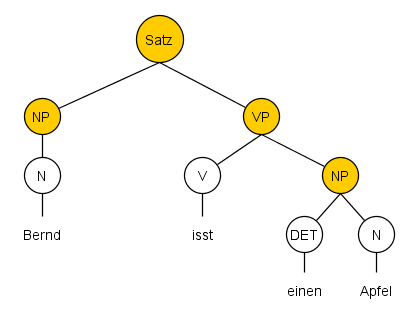
\includegraphics[width=11cm, height=8cm]{Grafiken/Ableitungsbaum}
		\end{figure}
		

	\subsection{Beispiel für eine mehrdeutige Grammatik}
		
		\begin{enumerate}[label={(\arabic*)}]
			\item{S $\rightarrow$ SUBJEKT PRÄDIKAT}
			\item{SUBJEKT $\rightarrow$ SUBSTANTIV}
			\item{SUBJEKT $\rightarrow$ ARTIKEL SUBSTANTIV}
			\item{SUBJEKT $\rightarrow$ ADJEKTIV SUBSTANTIV}
			\item{SUBJEKT $\rightarrow$ ARTIKEL ADJEKTIV SUBSTANTIV}
			\item{SUBJEKT $\rightarrow$ PERSONALPRONOMEN}
			\item{PRÄDIKAT $\rightarrow$ VERB}
			\item{PRÄDIKAT $\rightarrow$ VERB OBJEKT}
			\item{OBJEKT $\rightarrow$ SUBSTANTIV}
			\item{OBJEKT $\rightarrow$ ARTIKEL SUBSTANTIV}
			\item{OBJEKT $\rightarrow$ ADJEKTIV SUBSTANTIV}
			\item{OBJEKT $\rightarrow$ ARTIKEL ADJEKTIV SUBSTANTIV}
			\item{OBJEKT $\rightarrow$ PERSONALPRONOMEN}
		\end{enumerate}
		
		Aus: Höppner, Wolfgang (2004): \emph{">Unterlagen zur Vorlesung Algorithmen und formale Sprachen"<}.
			 URL: http://www.uni-due.de/imperia/md/content/computerlinguistik/algfs\_2002\_01.pdf [Stand: 17.03.2013]
			 Seiten 3 und 4.

	\subsection{Beispiel für eine probabilistisch-kontextfreie Grammatik}
	
		\begin{enumerate}[label={(\arabic*)}]
			\item{S $\rightarrow$ NP VP  (1.0)}
			\item{PP $\rightarrow$ P NP  (1.0)}
			\item{VP $\rightarrow$ V NP  (0.7)}
			\item{VP $\rightarrow$ VP PP (0.3)}
		\end{enumerate}
	
		S – Startsymbol; NP – Subjekt; VP – Prädikat; V – Verb; PP – Präpositionalphrase; P – Präposition
		
		In den Klammern stehen die Wahrscheinlichkeiten für jede Produktionsregel. Die Wahrscheinlichkeiten für alle Produktionen mit dem selben Ausgangssymbol müssen sich zu 1 aufaddieren.

	\subsection{Durchlauf des Marcus-Parsers}
		Schritt für Schritt Erläuterungen zur syntaktischen Analyse von ">Bernd isst einen Apfel"<\footnote{Dieses Beispiel entspricht ist leicht verändert aus [Fedzechkina und Schmidt 2008] übernommen, die Ausführungen sind jedoch von mir.}, unter Verwendung des Marcus-Parsers
		und der Grammatik $G$:
		
		\begin{enumerate}[label={(\arabic*)}]
			\item{S $\rightarrow$ NP VP}
			\item{NP $\rightarrow$ DET N}
			\item{NP $\rightarrow$ N}
			\item{VP $\rightarrow$ V}
			\item{VP $\rightarrow$ V NP}
			\item{VP $\rightarrow$ V PP}
			\item{PP $\rightarrow$ P NP}
		\end{enumerate}
		
		Aus Gründen der Übersichtlichkeit werden die Teilstrukturen des Baums durch ihr Wurzel-Symbol abgekürzt.
		Somit wird strenggenommen eigentlich nur entschieden ob die Eingabe zu $L(G)$ gehört, ein Syntaxbaum kann so nicht erstellt werden. Es ist aber ersichtlich, dass der Schritt vom Akzeptor zum richtigen Parser nur aus dem Speichern der Zwischenergebnisse besteht.\\

		\textbf{Stack: S\\
				Puffer: Bernd | isst | einen\\
		}
		Zu Beginn des Vorgangs ist die nächste erwartete Konstituente S, also das Startsymbol der Grammatik.
		Es existiert eine eindeutige Regel für S in G, nämlich (1). Somit fügen wir NP in den Erwartungsstack ein.
		Das erste Token im Puffer, ">Bernd"<, wird zudem als Nomen erkannt und kann durch das entsprechende POS-Tag N ersetzt werden.\\
		
		\textbf{Stack: S | NP\\
				Puffer: N | isst | einen\\
		}
		Nun ist NP also das aktive Symbol. Hierfür enthält $G$ zwei mögliche Regeln. Wir schauen also in den Puffer und finden dort ein N vor. Somit ist eindeutig, dass nur Regel (3) anwendbar ist. Wir erkennen weiterhin, dass die NP Teilstruktur hiermit abgeschlossen ist und vom Stack genommen werden kann (der Parser würde die Teilstruktur nun im Syntaxbaum an S ">hängen"< und abspeichern). Die Eingabe kann nun einen Platz weiter in den Puffer vorrücken.\\
		
		\textbf{Stack: S(1)\\
				Puffer: isst | einen | Apfel\\
		}
		S(1) soll hierbei bedeuten, dass wir eine Substruktur von S bereits bestimmt haben. Laut Regel (1) müsste nun eine Verbphrase (VP) folgen. Diese wird auf den Stack gelegt. Das nächste Symbol im Puffer, ">isst"<, wird als Verb (V) erkannt.\\
		
		\textbf{Stack: S(1) | VP\\
				Puffer: V | einen | Apfel\\
		}
		Aus $G$ gehen wieder mehrere mögliche Ableitungen für eine VP hervor. Das erste Symbol ist jedoch immer ein Verb. Wir schauen in den Puffer und erkennen dort das Verb. An dieser Stelle verwenden wir vorausschauendes Arbeiten: Wir erkennen, dass das zweite Token im Puffer, ">einen"<, auch zu einer VP gehören kann. Deswegen schließen wir diese nicht, sondern fügen ihr nur das bereits erkannte Verb an. ">einen"< wird derweil als Artikel markiert (DET - determiner).\\
		
		\textbf{Stack: S(1) | VP(1)\\
				Puffer: DET | Apfel\\
		}
		In diesem Schritt zeigt sich nun, warum der Marcus-Parser teilweise bottom-up operiert. Um nämlich entscheiden zu können, welche der drei Regeln (4), (5) oder (6) anzuwenden ist, betrachten wir das erste Puffersymbol, einen Artikel. Wir suchen nun in $G$ nach Ableitungen, die zu DET führen können.
		Die einzige passende Regel ist (2). Das bedeutet, dass die nächste erwartete Konstituente eine Nomenphrase sein muss.\\
		
		\textbf{Stack: S(1) | VP(1) | NP\\
				Puffer: DET | Apfel\\
		}
		Im Puffer befindet sich noch DET, welches nun  an die NP angehängt werden kann. Aus Regel (2) folgt weiter, dass nun ein Nomen folgen muss. Wir platzieren also ein N auf dem Stack. ">Apfel"< wird als N erkannt.\\
		
		\textbf{Stack: S(1) | VP(1) | NP(1) | N\\
				Puffer: N\\
		}
		Im Puffer befindet sich nun natürlich das erwartete Nomen, wir können also die N Struktur abschließen und auf den Puffer legen. Daraufhin erkennt die NP ihr fehlendes N und wird ebenfalls abgeschlossen. Wir verbleiben mit:\\
		
		\textbf{Stack: S(2)\\
				Puffer:\\
		}
		Es befindet sich nun nur noch das vollständig abgearbeitete Startsymbol auf dem Stack. Damit gehört die Eingabe zu $L(G)$. Im Parser befindet sich nun anstelle eines Symbols ein ganzer Ableitungsbaum (mit Wurzel S) auf dem Stack.
		
	\subsection{Google Knowledge Graph}
		\begin{figure}[hbtp]
		\centering
		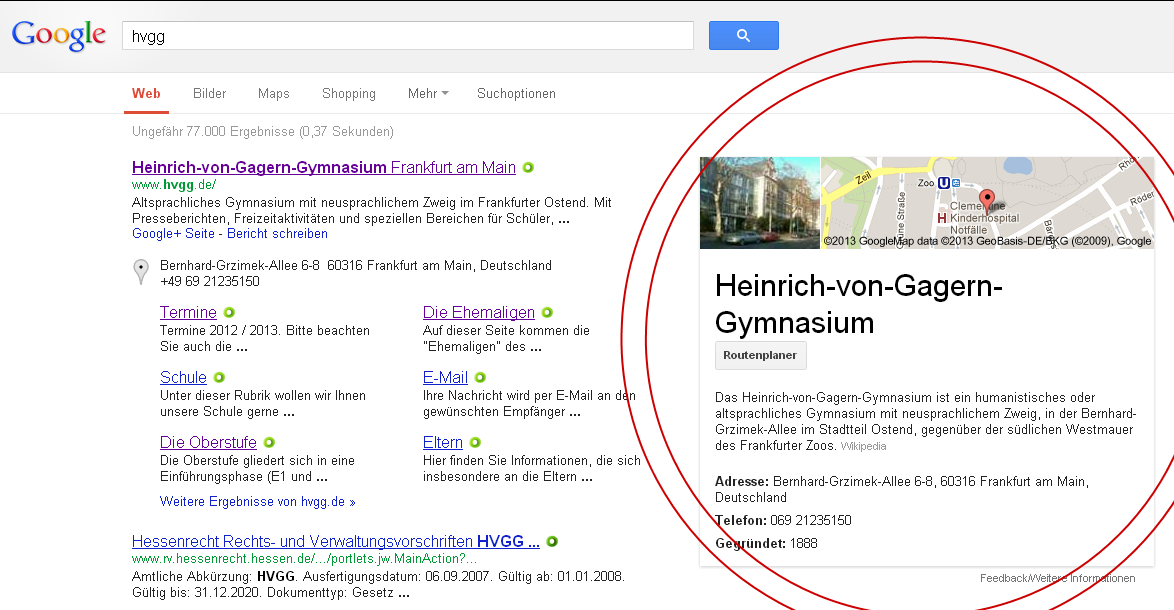
\includegraphics[width=\linewidth]{Grafiken/Google-Knowledge-Graph}
		\end{figure}
		
		\newpage

	\subsection{Beispiele für den Ngram Viewer}
		Der Ngram Viewer unterstützt mehrere Operationen. Die simpelste zählt die Vorkommen sogenannter n-Gramme, Textfragmente (Wortfolgen) der Länge n:
		Ich benutze hierbei den Korpus ">German 2012"<.
		
		\textbf{Auftreten von ">Krieg"< (blau) und ">Frieden"< (rot) von 1880 – 1980}
		\begin{figure}[hbtp]
		\centering
		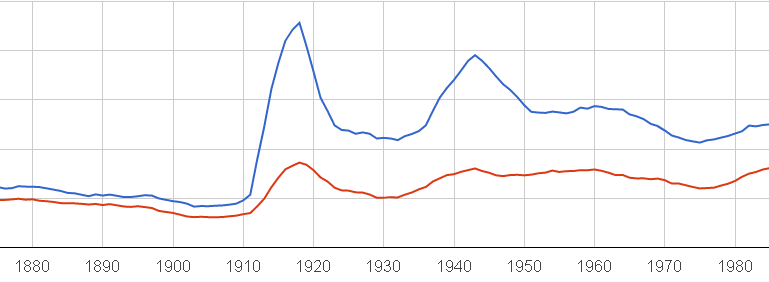
\includegraphics[width=\linewidth]{Grafiken/Krieg-vs-Frieden}
		\end{figure}
		
		Es ist sofort ersichtlich das von 1910-1920 sowie 1940-1945 die beiden Begriffe weitaus häufiger benutzt werden als in den Jahren davor und danach. Könnte zu diesen Zeiten in Deutschland etwas vorgefallen sein was diese Entwicklung hervorrief...? Auch wenn die Erklärung in diesem Falle offensichtlich ist, so scheint Krieg schon immer ein beliebteres Thema als Frieden gewesen zu sein.
		
		\textbf{Auftreten von ">Mann"< (blau) und ">Frau"< (rot) von 1900-2000}
		\begin{figure}[hbtp]
		\centering
		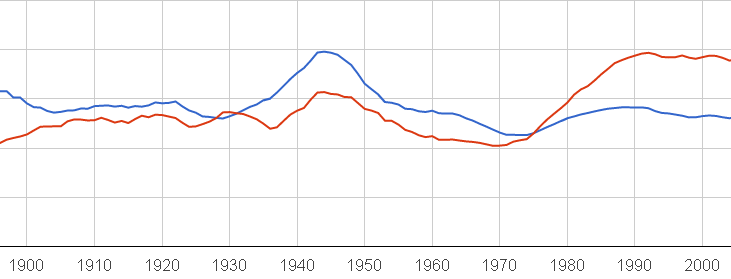
\includegraphics[width=\linewidth]{Grafiken/Mann-vs-Frau}
		\end{figure}
		
		Aktuelle politische Affären könnten durchaus Anlass zur Beschäftigung mit der Stellung von Mann und Frau in der Gesellschaft darstellen. Ein erstes Indiz: Das männliche Geschlecht, dem für Jahrhunderte die höhere Aufmerksamkeit im geschriebenen Wort galt, wurde schon 1975 von der Frau überholt. Eine detaillierte, geschweige denn eine kritische Auseinandersetzung mit diesen Themen will und kann an dieser Stelle nicht erfolgen, doch hoffe ich, dass die Möglichkeiten dieses kinderleicht zu bedienenden Werkzeugs aufgezeigt werden.
		
		Diese Analysen benötigen auf den ersten Blick eher Rechenleistung als das Verständnis von natürlicher Sprache, schließlich muss der Computer nur zählen. Doch die eigentliche Leistung der Maschinen ist nicht das zählen, sondern das sogenannte OCR (Optical Character Recognition), also das Erkennen von Text auf den Bildern, die Google's Scanner ihnen liefern. Denn mit einem Bild an sich weiß ein Rechner herzlich wenig anzufangen, erst komplexe Algorithmen können den darauf abgebildeten Text als solchen erkennen und auslesen.

\section{Source Code}
	Beide aufgeführte Programme benötigen eine, ebenfalls von mir geschriebene, Hilfsroutine zum Laden von Grammatiken aus Textfiles. Diese ist in der Datei code/grammar.py enthalten und hier nicht weiter aufgeführt.

	\subsection{Marcus-Parser (code/marcus.py)}
	Der Algorithmus ist in Pyhton 2.7 implementiert und benötigt das NLTK Modul (für die Darstellung der Syntaxbäume).
	Hier aufgeführt ist lediglich der Teil des Codes, der den Marcus-Algorithmus implementiert sowie benötigte Hilfsroutinen. Einige sonstige Zeilen, wie z.B. Benutzer-Eingabe wurde zur besseren Übersicht weggelassen.

	\singlespacing
	\begin{minted}{python}
from grammar import load_grammar

from nltk.tree import *
from nltk.draw import tree

# Ein assoziatives Array, das den Terminalen 
# ihr POS-Tag zuordnet.
__TERMINALS__ = {
  'Bernd': 'N',
  'Marcus': 'N',
  'Noam': 'N',
  'Apfel': 'N',
  'Paper': 'N',
  'Ball': 'N',
  'isst': 'V',
  'schneidet': 'V',
  'wirft': 'V',
  'schreibt': 'V',
  'den': 'DET',
  'einen': 'DET',
  'ein': 'DET',
  'der': 'P',
  'die': 'P',
  'das': 'P'
}

# Diese Routine gibt den Inhalt des Stacks s als String aus
def print_stack(s):
  _s_ = 'Stack: '
  for node in s:
    _s_ += '%s(%s) | ' % (node.root, node.pos)
  
  print _s_[:-2]

# Diese Routine gibt den Inhalt des Puffers b als String aus
def print_buffer(b):
  print('Buffer: %s' % " | ".join([str(x) for x in b]))

# Diese Funktion sucht, von einem Terminal s ausgehend,
# nach Produktionen in G die zu s fuehren.
# Dies ist die bottom-up Komponente des Marcus-Parsers.
def trace(s, to, G):
  #print("Tracing %s to %s" % (s,to))

  if s == to:
    return True

  for root, rules in G.iteritems():
    for rule in rules:
      if s in rule:
        if trace(root, to, G) == True:
          return True

  return False

# Diese Funktion filtert eine Grammatik G nach Produktionen die direkt zu s fuehren
def filter_rules(s, G):
  for root, rules in G.iteritems():
    for rule in rules:
      #print("%s in %s" % (s, rule))
      if s in rule:
        return root

  return None

# Die Node-Klasse repraesentiert einen Knoten des Syntaxbaums
class Node:
  def __init__(self, root, pos, childs=[]):
    self.root = root
    self.pos = pos
    self.node = Tree(self.root, childs)

  def __str__(self):
    return self.root

# Diese Funktion implementiert den Marcus-Parser mit lookahead = 3.
# !Bitte beachten: Fuer k != 3 operiert der Algorithmus noch fehlerhaft!
def marcus(w, G, k=3):
  w = w.split(' ') # Zerlegung der Eingabe in Tokens

  # Initialisieren des Stacks und des Puffers
  stack = []
  buf = w[:3]
  w_i = 0 # Position in der Eingabe, zu Beginn = 0

  # Wir fuegen dem Stack den Wurzelknoten an
  stack.append( Node(G['__root__'], 0) )
  
  while True:
    print('---------------------------------------')
    print_stack(stack)
    print_buffer(buf)
    
    # Das naechste erwartete Symbol wird vom Stack genommen
    active = stack.pop()
    position = active.pos
    new_pos = active.pos

    print('Active: %s\n' % active.root)
    
    if active.root in G: # Das aktive Symbol ist ein Nichterminal
      rules = G[active.root] # Alle moeglichen Regeln von diesem NT aus
      
      if rules == []:
        print("Es existieren keine Regeln fuer dieses Nichtterminal!")
        return None # Ergo kann w nicht in L(G) sein

      # Wir pruefen ob das naechste Element im Puffer ein Terminal ist
      buf_0 = buf[0]
      if buf_0 in __TERMINALS__:
        # Dies ist der Fall, wir ersetzen das erwartete Terminal an dieser
        # Stelle durch das korrespondierende POS-Tag
        
        buf_0 = Node(__TERMINALS__[buf_0], 0, [buf_0])
        buf[0] = buf_0

      # Wir durchlaufen nun alle moeglichen Produktionen fuer das aktive Symbol
      rule_found = False
      for rule in rules:

        # koennen wir uns innerhalb dieser Regel befinden?
        # und entspricht das naechste Symbol im Puffer dieser Regel?
        
        if active.pos < len(rule) and buf_0.root == rule[active.pos]:
          new_pos += 1
                    
          if new_pos >= len(rule): # Befinden wir uns am Ende der Regel?
            
            # Ja, das heisst, wir muessen nun pruefen ob die aktive Teilstruktur
            # ebenfalls abgeschlossen werden kann.
          
            if len(buf) < 2 or trace(__TERMINALS__[buf[1]], active.root, G) == False:
              
              # Das uebernaechste Element im Puffer kann unmoeglich durch
              # das aktive produziert werden. (Dies ist natuerlich auch erfuellt
              # wenn weniger als 2 Elemente im Puffer sind.)
              
              # Die aktive Teilstruktur kann geschlossen..
              active.node.append(buf[0].node)
              buf[0] = active # ...und das aktive Puffer Element ersetzen.
            
            else:
              # Diese Teilstruktur ist noch nicht beendet
              # und muss wieder an den Stack erwarteter Symbole angefuegt werden

              active.node.append(buf[0].node)

              w_i += 1
              buf = w[w_i:w_i+3]
              
              active.pos = new_pos
              stack.append(active)
              
              # zudem suchen wir nun nach dem naechsten Symbol,
              # dass unsere unvollstaendige Struktur komplettiert.
              stack.append( Node(filter_rules(__TERMINALS__[buf[0]], G), 0) )
            
          else:
            # Diese Produktion ist noch nicht beendet,
            # wir fuegen also einfach das passende naechste Symbol an
            # unseren aktuellen Knoten an...

            active.node.append(buf[0].node)

            # ...und lassen das naechste Symbol der Eingabe
            # in den Puffer nachruecken
            w_i += 1
            buf = w[w_i:w_i+3]

            active.pos = new_pos
            stack.append(active)

          rule_found = True
          break    

      if rule_found == False:
        # Wir konnten keine einzige eindeutige Regel finden,
        # muessen also nun bottom-up erwartete Symbole generieren
        stack.append(active)
        
        rule = rules[0]
        #print("%s (%s)" % (" ".join(rule), position))
        stack.append( Node(rule[position], 0) )

      #print("Found rule %s -> %s" % (active.root, " ".join(rule)))

    if len(stack) == 0:
      if len(buf) == 1:
        # Es befindet sich nur noch ein Knoten im Puffer, der vollstaendige
        # Syntaxbaum.
        return buf[0].node
      return None

    #raw_input()

  print("Es wurde kein Syntaxbaum gefunden.")
  return None
	\end{minted}

	\subsection{Earley-Akzeptor (code/earley.py)}
		Zuletzt noch meine Implementation des Earley-Akzeptors (kein Syntaxbaum wird generiert). Diese ist ebenfalls in Python 2.7 verfasst.

		\singlespacing
		\begin{minted}{python}
# In dieser Funktion ist der Earley-Akzeptor implementiert.
def earley(w, G, k=1):
  n = len(w)
  w += k*'#' # der Parser erkennt sonst das Ende der Eingabe nicht

  # Wir erstellen eine Liste mit State-Sets
  # und fuegen den Startzustand ein.
  sets = [[] for x in range(n+2)]
  sets[0].append( (('S', G['__root__']+'#'*k), 0, '#'*k, 0) )

  s_i = 0
  while True:
    current_set = sets[s_i]
    print("\n\nSet %s:" % s_i)

    # Wenn das aktuelle Set leer ist wurde keine passenden Zustaende uebertragen.
    # w kann nicht in L(G) sein.
    if current_set == []:
      print("    Die Zustandsmenge ist leer. Die Eingabe ist nicht in L(G).")
      return False

    for q in current_set:
      P = q[0] # auftrennen des Zustands-Tupels in handhabbare Variablen
      i = q[1]
      l = q[2]
      s = q[3]

      # Ausgabe des Zustands
      print("    %s" % rule_to_str(P[0], P[1], i))

      # Haben wir das Ende der Produktion erreicht?
      if i == len(P[1]):

        # Ja, wir muessen also pruefen ob es moeglich ist sie abzuschliessen.
        
        # Wenn der lookahead den naechsten k Symbolen der Eingabe entspricht
        # darf der completer verwendet werden.
        if l == w[s_i:s_i+k]:

          # [COMPLETER]
          # Wir pruefen alle alten Sets auf Zustaende 
          # die zu dem aktuellen gefuehrt haben.
          for old_q in sets[s]:
            rule = old_q[0]
            pos = old_q[1]
            lookahead = old_q[2]
            origin = old_q[3]

            if P[0] == peek(rule[1], pos, lookahead):
              q_new = (rule, pos+1, lookahead, origin)
              current_set.append(q_new)
              
          # [/COMPLETER]

      else:
        next_symbol = peek(P[1], i, l)

        # Ist das naechste Symbol ein Nichtterminal?
        if next_symbol in G.keys():

          # [PREDICTOR]
          # Wir fuegen alle auf das Symbol anwendbaren Regeln
          # in die aktuelle Zustandsmenge ein.
          for rule_body in G[next_symbol]:
            q_new = ((next_symbol, rule_body), 0, peek(P[1], i+k, l), s_i)
            if q_new not in current_set:
              current_set.append(q_new)
          # [/PREDICTOR]

        # Oder ist ein Terminal das naechste Symbol?
        elif (next_symbol == peek(w, s_i, '#')) or (next_symbol == '#'): 

          # [SCANNER]
          # Der Scanner kopiert diesen Zustaend ins naechste Set.
          q_new = (P, i+1, l, s)
          sets[s_i+1].append(q_new)
          # [/SCANNER]

    # Ist der Anfangszustand abgeschlossen?
    if (len(current_set) == 1) and
     	(current_set[0] == (('S', G['__root__']+'#'*k), 2, '#'*k, 0)):
      # Dann ist w in L(G)
      return True

    s_i += 1

  return False
		\end{minted}

	\subsection{Grammatiken (code/grammars)}
		Die beiden verwendeten Grammatiken sind hier nochmal aufgeführt.

		\subsubsection{marcus.gr}
			\begin{enumerate}[label={(\arabic*)}]
				\item{S $\rightarrow$ NP VP}
				\item{NP $\rightarrow$ DET N}
				\item{NP $\rightarrow$ N}
				\item{VP $\rightarrow$ V}
				\item{VP $\rightarrow$ V NP}
				\item{VP $\rightarrow$ V PP}
				\item{PP $\rightarrow$ P NP}
			\end{enumerate}
		
		\subsubsection{earley.gr}
			Dies ist die Grammatik aus [Earley 1968]. Sie beschreibt Produkte und Summen mit dem Symbol a.
			
			\begin{enumerate}[label={(\arabic*)}]
				\item{E $\rightarrow$ T}
				\item{E $\rightarrow$ E + T}
				\item{T $\rightarrow$ P}
				\item{T $\rightarrow$ T * P}
				\item{P $\rightarrow$ a}
			\end{enumerate}

\newpage
	
\begin{thebibliography}{99}
	\bibliographystyle{plainnat}
	\thispagestyle{empty}
	\raggedright
	
	\bibitem{aho1975}
		Aho, Johnson und Ullman (1975):
		\emph{">Deterministic Parsing of Ambiguous Grammars"<}.\\
		URL: http://lambda.csail.mit.edu/~chet/papers/others/a/aho/aho73popl.pdf \\
		{[Stand: 19.01.2013]}
	
	\bibitem{chater2006}
		Chater, Nick und Manning, Christopher D. (2006):
		\emph{">Probabilistic models of language processing and acquisition"<}.\\
		URL: http://www.stanford.edu/class/linguist1/Rdgs/chater.pdf\\
		{[Stand: 16.03.2013]}
	
	\bibitem{chomsky1956}
		Chomsky, Noam (1956):
		\emph{">Three Models for the Description of Language"<}.\\
		URL: http://stevereads.com/papers\_to\_read/three\_models\_for\_the\_description\_of\_language.pdf\\
		{[Stand: 12.01.2013]}

	\bibitem{chomsky1957}
		Chomsky, Noam (1972):
		\emph{Syntactic Structures.}
		10. Auflage
		Den Haag: Mouton \& Co. [1. Aufl. 1957]

	\bibitem{chomsky1993}
		Chomsky, Noam (1993):
		\emph{">The Minimalist Program"<}.\\
		URL: http://books.google.de/books?id=vtPQiYCNpjgC\\
		{[Stand: 12.01.2013]}

	\bibitem{covington1990}
		Covington, Michael A. (1990):
		\emph{">Parsing Discontinuous Constituents in Dependency Grammar"<}.\\
		URL: http://delivery.acm.org/10.1145/130000/124997/p234-covington.pdf\\
		{[Stand: 13.01.2013]}

	\bibitem{durdaut2012}
		Durdaut, Rainer (2012):
		\emph{">Automatentheorie, Berechenbarkeit, Formale Sprachen"<}.\\
		Skript zum Informatikunterricht 2012/13.

	\bibitem{earley1968}
		Earley, Jay (1968):
		\emph{">An Efficient Context-Free Parsing Algorithm"<}.\\
		URL: http://reports-archive.adm.cs.cmu.edu/anon/anon/usr/ftp/scan/CMU-CS-68-earley.pdf\\
		{[Stand: 17.02.2013]}

	\bibitem{fedzechkina2008}
		Fedzechkina, Maryia und Schmidt, Frauke (2008):
		\emph{">Der Marcus-Parser"<}.\\
		URL: http://www.spinfo.phil-fak.uni-koeln.de/uploads/media/MarcusParser.pdf\\
		{[Stand: 28.12.2012]}

	\bibitem{hale2001}
		Hale, John (2001):
		\emph{">A Probabilistic Earley Parser as a Psycholinguistic Model"<}.\\
		URL: http://acl.ldc.upenn.edu/N/N01/N01-1021.pdf\\
		{[Stand: 10.02.2013]}

	\bibitem{hermes2012}
		Hermes, Jürgen (2012):
		\emph{">Computerlinguistische Grundlagen"<}.\\
		URL: http://www.spinfo.phil-fak.uni-koeln.de/fileadmin/spinfo/cl/CL\_10.pdf\\
		{[Stand: 05.02.2013]}

	\bibitem{hindle1983}
		Hindle, Donald (1983):
		\emph{">Deterministic Parsing Of Syntactic Non-Fluencies"<}\\
		URL: http://clair.eecs.umich.edu/aan/paper.php?paper\_id=P83-1019\#pdf\\
		{[Stand: 16.03.2013]}

	\bibitem{joshi1991}
		Joshi, Aravind K. [et. al.] (1991):
		\emph{">The Convergence of Mildly Context-Sensitive Grammar Formalisms"<}.\\
		URL: http://citeseerx.ist.psu.edu/viewdoc/download?doi=10.1.1.178.7432\&rep=rep1\&type=pdf\\
		{[Stand: 19.02.2013]}
	
	\bibitem{jaeger2008}
		Jäger, Gerhard (2008):
		\emph{">Formale Methoden 1"<}.\\
		URL: http://www.sfs.uni-tuebingen.de/~gjaeger/lehre/ws0708/fm1/folien10.pdf\\
		{[Stand: 24.02.2013]}

	\bibitem{kallmeyer2010}
		Kallmeyer, Laura (2010):
		\emph{Parsing Beyond Context-Free Grammars.}
		1. Auflage
		Heidelberg: Springer (Cognitive Technologies)
	
	\bibitem{kallmeyer2009}
		Kallmeyer, Laura und Maier, Wolfgang (2009):
		\emph{An Incremental Earley Parser for Simple Range Concatenation Grammar}.\\
		URL: http://www.aclweb.org/anthology-new/W/W09/W09-3808.pdf\\
		{[Stand: 22.02.2013]}
	
	\bibitem{laput2013}
		Laput, Gierad [et. al.] (2013):
		\emph{">PixelTone: A Multimodal Interface for Image Editing"<}.\\
		URL: http://www.cond.org/pixeltone.pdf\\
		{[Stand: 21.02.2013]}
	
	\bibitem{li2009}
		Li, Te und Alagappan, Devi (2009):
		\emph{">A Comparison of CYK and Earley Parsing Algorithms"<}.\\
		URL: http://150.145.63.3/ruffolo/progetti/projects/09.Parsing CYK/A Comparison of CYK and Earley Parsing Algorithms-cykeReport.pdf\\
		{[Stand: 17.02.2013]}
	
	\bibitem{marcus1980}
		Marcus, Mitchell P. (1986):
		\emph{A Theory of Syntactic Recognition for Natural Language.}
		4. Auflage
		Massachussetts: The MIT Press. [1. Aufl. 1980]

	\bibitem{mukherjee2012}
		Mukherjee, Arjun [et. al.] (2012):
		\emph{Spotting Fake Reviewer Groups in Consumer Reviews}.\\
		URL: http://www.cs.uic.edu/~liub/publications/WWW-2012-group-spam-camera-final.pdf\\
		{[Stand: 10.01.2013]}

	\bibitem{nivre2004}
		Nivre, Joakim (2004):
		\emph{Incrementality in Deterministic Dependency Parsing}.\\
		URL: http://acl.ldc.upenn.edu/W/W04/W04-0308.pdf\\
		{[Stand: 19.01.2013]}

	\bibitem{petersen2006}
		Petersen, Wiebke (2006):
		\emph{">The formal Complexity of Natural Languages"<}.\\
		URL: http://user.phil-fak.uni-duesseldorf.de/~petersen/Riga/print\_Folien\_Riga\_complexity\_new.pdf\\
		{[Stand: 06.02.2013]}

	\bibitem{petersen2010}
		Petersen, Wiebke (2010):
		\emph{">Einführung in die Computerlinguistik. Zusammenfassung."<}.\\
		URL: http://user.phil-fak.uni-duesseldorf.de/~petersen/Einf\_CL/ECL\_Zusammenfassung.pdf\\
		{[Stand: 04.02.2013]}

	\bibitem{shiber1985}
		Shieber, Stuart (1985):
		\emph{">Evidence Against the Context-Freeness of Natural Language"<}.\\
		URL: http://www.eecs.harvard.edu/~shieber/Biblio/Papers/shieber85.pdf\\
		{[Stand: 09.01.2013]}
	
	\bibitem{stolcke1995}
		Stolcke, Andreas (1995):
		\emph{">An Efficient Probabilistic Context-Free Parsing Algorithm that Computes Prefix Probabilities"<}.\\
		URL: http://dl.acm.org/citation.cfm?id=211197\&bnc=1\\
		{[Stand: 22.02.2013]}
	
	\bibitem{wegener1999}
		Wegener, Ingo (1999):
		\emph{Theoretische Informatik - eine Algorithmische Einführung.}
		2. Auflage
		Stuttgart, Leipzig.: B.G. Teubner

\end{thebibliography}

\onehalfspacing

\section{Arbeitstagebuch}
	Im Folgenden sind die einzelnen Etappen dieser Arbeit zusammengefasst aufgezeichnet. Insgesamt betrug die Arbeitszeit knapp 140 Stunden.
	Bei den Recherchen wurden etwa 60 wissenschaftliche und nochmal so vielen andere Quellen durchgesehen.

	\textbf{September und Oktober 2012}
		Allgemeine Recherche, Experimente mit dem Python NLTK.
		Insgesamt knapp 10 Stunden.

	\textbf{November und Dezember 2012}
		Intensive Lektüre und Strukturierung des Materials.
		Anlegen einer ">Datenbank"< an Begriffen, Themen und Gedankengängen.
		Beginn der schriftlichen Rohfassung I.
		Frequenz ab Heiligabend: Ein bis zwei Stunden täglich, davor seltener.
		Insgesamt wenigstens 10-12 Stunden.
		
		Stand gegen Ende Dezember: 500 Wörter und etwa 10\% des Inhalts.

	\textbf{Januar 2013}
		Arbeit in regelmäßigen Abständen von etwa drei Tagen, knapp über zwei Stunden am Tag.
		Intensives Schreiben. Themen: POS-Tagging, Gesellschaftliche Relevanz, Chunking, Parsing, Marcus-Parser, Determinismus und Nichtdeterminismus.
		Recherche zu SKS-Grammatiken und Komplexitätsanalysen.
		Strukturierung und Aufbau.
		Insgesamt wenigstens 20 Stunden.
		
		Stand gegen Ende Januar: Knapp 4000 Wörter und 75\% des geplanten Inhalts. Rohfassung I nahezu fertig.
		
	\textbf{Februar 2013}
		Weitere Recherchen. Daraus resultierend: Verwerfung großer Teile der Rohfassung I (~2000 Wörter).
		Frequenz: Nahezu täglich, zwei bis vereinzelt sechs Stunden. Zwei Pausen für mehrere Tage. Neue Struktur und Festhalten bisheriger Erkenntnisse. Arbeit an der Einführung, abarbeiten der neu-strukturierten Kapitel. Fertigstellung des vierten Kapitels und Implementation der Programme.
		Insgesamt wenigstens 70 Stunden.
		
		Stand gegen Ende Februar: Etwas über 6000 Wörter und 70-80\% des geplanten Inhalts. Rohfassung II nahezu fertig.
	
	\textbf{März 2013}
		Arbeit in unregelmäßigen Abständen, drei bis vier Stunden am Tag. Transfer der Arbeit zu LaTeX. Fertigstellung des Anhangs und der Bibliographie, korrigieren von Feinheiten. Insgesamt etwas über 20 Stunden.

\section{Danksagungen}
	Danken möchte ich zunächst einmal meinem Lehrer Herrn Durdaut, der diese Arbeit betreut hat. Weiterhin meinem Vater, für interessante Diskussionen zur Linguistik im Allgemeinen und für das Aufzeigen vieler kleiner Ecken und Kanten, meinem BLL-Kollegen Peter Fürstenau, der mir mit nützlichen Tipps, vor allem zum Umgang mit LaTeX, einiges erleichtert hat. Danke auch an meine Freundin, einmal fürs Fehlerlesen und für die moralisch-seelische Unterstützung. Und zuletzt noch Julius Frank, für präzise gefaltete Kraniche. Vielen Dank.

\end{document}